\documentclass{ximera}

\newcommand{\N}{\mathbb{N}}
\newcommand{\Z}{\mathbb{Z}}
\newcommand{\Q}{\mathbb{Q}}
\newcommand{\F}{\mathbb{F}}
\newcommand{\I}{\mathbb{I}}
\newcommand{\R}{\mathbb{R}}
\newcommand{\C}{\mathbb{C}}
\renewcommand{\P}{\mathbb{P}}
\renewcommand{\O}{\mathbb{O}}

\newcommand{\x}{\boldmath{x}}

\newcommand{\citep}{\cite}


\newcommand{\red}{\color{red}}
\newcommand{\black}{\color{black}}
\newcommand{\magenta}{\color{magenta}}

\newcommand{\BEx}{\begin{exercise}} 
\newcommand{\EEx}{\end{exercise}} 
\newcommand{\sol}[1]{\begin{solution}#1\end{solution}}    
\newcommand{\bbm}{\begin{bmatrix}} \newcommand{\ebm}{\end{bmatrix}}
\newcommand{\be}{\begin{equation}} \newcommand{\ee}{\end{equation}}
\newcommand{\Be} {\begin{enumerate}} \newcommand{\Ee}{\end{enumerate}}
\newcommand{\Caption}[1]{\caption{\footnotesize \setlength{\baselineskip}{.5em} \sl #1}}


%% BART: Ximera does not allow labels to be inside of headings. 
%% Solution: Move them just below headings

%Chapter 2

%Format for subsection:
\title  %[Stream 1: Number Systems ]
	{Stream 1: Number Systems}
%\setcounter{exercise}{0} %% BART

\begin{document}
\begin{abstract}
\end{abstract}
\maketitle
\label{Chap:NS} \label{Sect:NS}
\index{stream 1}

Number theory (the study of numbers) was a starting point for many key ideas.
For example, in Euclid's geometrical constructions the Pythagorean theorem for real numbers $[a,b,c]$ was accepted as true,
but the emphasis in the early analysis was on integer constructions, such as Euclid's formula for Pythagorean triplets (Eq.~\ref{eq:EuclidsFormula}, p.~\pageref{eq:EuclidsFormula}).
 %Fig.~\ref{fig:bricks}, 

 \index{Pythagorean triplets} %\index{composition}
\index{Fibonacci recursion formula}
As we shall see, the derivation of the formula for Pythagorean triplets is the first of a rich body of
mathematical constructions---such as solutions of Pell's equation (p.~\pageref{Lec 8}),%
% BART \footnote {Heisenberg, an inventor of the matrix algebra form of quantum mechanics, learned mathematics
% by studying Pell's equation (p.~\pageref{Lec 8}) by eigenvector and recursive analysis methods. {\scriptsize \url{https://www.aip.org/history-programs/niels-bohr-library/oral-histories/4661-1}} \label{PellsEquation}
% \index{Pell's equation, Heisenberg's view}
% 	}
and recursive difference equations, such as solutions of the Fibonacci recursion formula
$f_{n+1} = f_n + f_{n-1}$ (see p.~\pageref{Lec 9})---that goes back at least to the Chinese (2000 BCE).
These are early pre-limit forms of calculus, best analyzed using an eigenfunction
(e.g., eigenmatrix) expansion, a geometrical concept from linear algebra, as an orthogonal set of
normalized unit-length vectors (see Appendix \ref{Apdx:Eigvector}, p.~\pageref{Apdx:Eigvector}).

%Format for subsection:
%\paragraph{The first use of zero and $\infty$:}
%{\magenta The first use of zero and $\infty$}

It is impossible to imagine that anyone who uses an abacus would fail to appreciate the concept of zero and
negative numbers. It does not take much imagination to go from counting numbers $\N$ to the set of
all integers $\Z$, including zero.  On an abacus, subtraction is obviously the inverse of addition. 
 %If five beads are moved up, and one is moved down, then four are left. Then if four more are
 %move down, that leaves zero.  Taking away (subtracting) is the opposite of giving (adding).
Subtraction to obtain zero abacus beads is no different from subtraction from zero, which gives
\emph{negative} beads.  To assume that the Romans, who first developed counting sticks, or the Chinese,
who then deployed the concept using beads, did not understand negative numbers, is simply not possible.
 \index{abacus}
However, understanding the concept of zero (and negative numbers) is not the same as having a symbolic
notation.  The Roman number system has no such symbols. 
The first recorded use of a symbol for zero is said to be by Brahmagupta in 628 CE.%BART\footnote{\scriptsize\url{https://news.nationalgeographic.com/2017/09/origin-zero-bakhshali-manuscript-video-spd/}; \scriptsize\url{https://www.nytimes.com/2017/10/07/opinion/sunday/who-invented-zero.html}}

% \footnote{The fall of the Roman Empire has been defined as Sept.~4, 476 {CE}.}
 \index{Brahmagupta}
However, this is likely wrong, given the notation developed by the Mayan civilization,
which existed from
2000 BCE to 900 CE.%BART\footnote{\scriptsize\url{https://www.storyofmathematics.com/mayan.html}}
There is speculation that the Mayans cut down so much of the Amazon jungle that it eventually resulted
in global warming, possibly leading to their demise.
  % interesting word of mouth via Phil Krein, ECE UIUC, Nov 2018

The definition of zero depends on the concept of subtraction, which formally requires the
creation of algebra (ca. 830 CE; see Fig.~\ref{fig:timelineBCE}, p.~\pageref{fig:timelineBCE}).
But apparently it took more than 600 years from the time Roman numerals were put into use, without
any symbol for zero, to the time the symbol for zero is first documented.
Likely this delay was more about the political situation, such as government rulings, than mathematics.

 %
%In summary, anyone capable of inventing the abacus, is capable of understanding the concept and
%representation of both zero and negative numbers.
 %All one has to do is loan money, and have a payback schedule, for the concepts to become intuitive.
 %

The concept that caused much more difficulty was $\infty$, or infinity, first proposed by Bernhard Riemann in 1851 with the
development of the extended plane, which mapped the plane to a sphere
(see Fig.~\ref{fig:ExtendedPlane}, p.~\pageref{fig:ExtendedPlane}). His construction made it clear that the point at $\infty$ is simply
another point on the open complex plane, since rotating the sphere (extended plane)
moves the point at $\infty$ to a finite point on the plane, thereby closing the complex plane.


\section {The taxonomy of numbers: $\P, \N, \Z, \Q, \F, \I, \R, \C$}% 
\label{Lec 2}
% {\magenta  First use of 0, $\infty$; Taxonomy of Numbers \\
%  Review of the fund theorems of math: Primes, Factoring Scalar Calc, Vect Calc; disc of integers }

Once symbols for zero and negative numbers were accepted, progress could be made. 
This led to the theory of numbers, today known as \emph{Number theory} \citep{HardyWright38,apostol2013}.

To fully understand numbers, a transparent notation is required. First one must identify the different classes (genus) of numbers, providing a notation that defines each of these
classes along with their relationships.
 %
It is logical to start with the most basic counting numbers, which we indicate with the double-bold symbol $\N$ (page \pageref{Symbols}).
 % (See Appendix \ref{Apdx:Notation}). 
For easy access, notation is summarized in Appendix \ref{Apdx:Notation}.
%double-bold symbols and set-theory symbols--that is,
% $\{\cdot\}, \cup, \cap, \in, \cancel{\in}, \perp$, and so on--

\paragraph{Counting numbers $\N$:}
\label{page:bbN} 


These are known as the \emph{natural numbers} $\N= \{1, 2, 3, \dots\}$ and denoted by the double-bold symbol
$\N$.  For clarity we shall refer to the natural numbers as \emph{counting numbers}, since \emph{natural},
which means \emph{integer}, is vague.  The mathematical sentence ``$2 \in \N$'' is read as
``2 is a member of the set of counting numbers.''
The word \emph{set} is defined as the collection of any objects that share a specific property.
Typically a set may be defined either by a sentence or by example.
 \index{counting numbers}
 \index{$\N$: see counting numbers}
 \index{Natural numbers: see counting numbers}

%Thus one may read the sentence as \emph{2 is a member of the collection of all counting numbers}.
%The number 2 and the genus $\N$ are two of the many nouns of the language of mathematics.


%Primes
\paragraph{Primes $\P$:}%

% \label{page:bbP} %} BART
% A number is prime ($\pi_n \in\P$) if its only factors are 1 and itself. %
%  % \footnote{40 primes are generated by the quadratic $P_k=k^2-k+41$, $k=1:40$. But why?}
% %Since $1= 1\cdot 1$, $1\not\in \P$, as it is seen to violate this basic definition of a prime. 
% The set of primes $\P$ is a subset of the counting numbers ($\P \subset \N$). A somewhat amazing
% fact, well known to the earliest mathematicians, is that every integer may be written as a unique
% product of primes. A second key idea is that the density of primes $\rho_\pi(N) \sim 1/\log(N)$; that is, $\rho_\pi(N)$ is inversely proportional to the log of $N$,
% 	%	 (Eq.~\ref{eq:PrimeDensity}, p.~\pageref{eq:PrimeDensity}),
% an observation first quantified by Gauss \citep{Goldstein73}.
% A third is that there is a prime between every integer $N\ge2$ and $2N$.  %, excluding $2N$. <-- why this?
% \index{primes} \index{$\P$: see primes}
%  %`
%  %we shall 'see this is a massively under estimate of the number of primes per octave (a factor of 2) as $n\rightarrow \infty).
%  \red
%  %
%  % this figure is @ /home/BACKUP/usr/local/UIUC/Springer/M/PrimeRatio.m and there should be a file: "PrimeRatio.pdf"
%  %
% In Fig.~\ref{fig:PrimeRatio} we shall show that this is a massive under estimate of the density of primes per octive (factor in 2 in $n$).
% %
% \index{prime number theorem}
% %\index{PNT: see prime number theorem}  %redundent
% A fourth fact is that the reciprocals of primes are \emph{fractional} ($1/\pi_k\in \F$), which are periodic in their representation.%
%  %\footnote{ \url{https://en.wikipedia.org/wiki/Reciprocals_of_primes}} BART
%  \black
% This does not seem to have reached the level of being declared a theorem, but perhaps the time has finally arrived.

% HELLO


% Below we use the notation $\pi_n$ for the prime numbers, indexed by $n\in\N$. 
% The first 12 primes are $\{n | 1 \le n \le 12\} = \{\pi_n | 2, 3, 5, 7, 11, 13, 17, 19, 23, 29, 31, 37 \}$.
% Since $4=2^2$ and $6=2 \cdot 3$ may be factored,  $4, 6 \not\in \, \P$ (read as ``4 and 6
% are not in the set of primes'').  Given this definition, multiples of a prime--that is, $[2, 3, 4, 5, \ldots] \times \pi_k$ of any prime $\pi_k$--cannot be prime.
% It follows that all primes except 2 must be odd, and that every integer $N$ is unique in its prime factorization.

HELLO

The ratio of primes $\pi_m/\pi_n$ is an interesting set with no special notation, such as $\O$.
An important special case are \emph{reciprical primes} $2/\pi_n\in \F$, which like $\pi_k$, are all unique.


HELLO

\BEx Write the first 20 integers in prime-factored form. 

\sol{\( 1, 2, 3, 2^2, 5, 2\cdot3, 7, 2^3, 3^2, 2\cdot 5, 11, 3\cdot 2^2,
13, 2\cdot7, 3\cdot5, 2^4, 17, 2\cdot 3^2, 19, 2^2\cdot5\)
%{\( 1, {\red 2}, {\red 3}, 2^2, {\red 5}, 2\cdot3, {\red 7}, 2^3, 3^2, 2\cdot 5, {\red 11}, 3\cdot 2^2,
%{\red 13}, 2\cdot7, 3\cdot5, 2^4, {\red17}, 2\cdot 3^2, {\red19}, 2^2\cdot5\). } 
}
\EEx
%\Exercise
\BEx
Write the integers $2$ to $20$ in terms of $\pi_n$. Here is a table to assist you:
\begin{center}
\begin{tabular} {l|cccccccccccc}
$n$ & 1& 2 & 3 &4&5&6&7&8&9&10&11&$\cdots$\\
\hline
$\pi_n$ & 2& 3& 5& 7&11 &13 &17 &19 &23 &29 & 31 &$\cdots$\\
\end{tabular}
\end{center}

 \sol{
\begin{center}
\begin{tabular} {l|ccccccccccccccc}
$n$ & 2 & 3 &4&5&6&7&8&9&10&11&12&13&14&$\cdots$\\
\hline
$\Pi\pi_n$&$\pi_1$&$\pi_2$ &$\pi_1^2$ &$\pi_3$ &$\pi_1 \pi_2$ &$\pi_4$
	&$\pi_1^3$ &$\pi_2^2$ &$\pi_1 \pi_3$ &$\pi_5$ &$\pi_1^2\pi_2$ &$\pi_6$ &$\pi_1\pi_4$&$\cdots$ \\
\end{tabular}
\end{center}
	}
\EEx

 \index{coprimes} \index{relatively prime, coprime)}
\emph{Coprimes} are two numbers that have no common factors. 
For example, $21=3\cdot 7$ and $10 = 2 \cdot 5$ are coprime, whereas $4=2\cdot2$ and $6=2\cdot 3$,
which have 2 as a common factor, are not coprime.  By definition all unique pairs of primes are coprime. 
We shall use the notation $m \perp n$ to indicate that $m$ and $n$ are coprime. The ratio of two coprimes
is \emph{reduced}, meaning it contains no factors to cancel.
The ratio of two numbers that are not coprime may always be reduced by canceling the common factors.
\emph{Gaussian primes} are of the form $\pi_k + \sqrt{-1}\pi_l$ for $k, l\in \N$, with $k \ne l$.
%
 %remove this footnote because it is both confusing and speculative.
 %\footnote{It is possible that Gaussian primes could be useful for generating security codes based on the pole location in the
 %complex plain. A pair of primes could have some coprimes that lead to interesting properties in the \LT. The pole location could
 %provide utility if the nature of the code security. These would be in the z-transform domain, and inside or outside the unit circle
 %could impact their lifetime, for example. \blue Newton's method for root location could be useful.}



When we do numerical work, for computational accuracy, it is always beneficial to work with coprimes.
Generalizing this idea, we define \emph{triprimes} as three prime numbers with no common factor,
such as \{$\pi_3, \pi_9, \pi_2$\}.
\index{reduced prime form}
\index{$\perp$: see perp p.~\pageref{Appx:perp}}

The \emph{fundamental theorem of arithmetic} states that every integer may be uniquely expressed as a unique product
of primes.  The \emph{prime number theorem} states the mean density of primes $\rho_\pi(n)$ as a function of $n\in\N$.
 \index{prime number theorem}

One of the more interesting properties of primes are that their reciprocals are rational ($\in\Q$).
 {\magenta
 I speculate that primes might also play a role in natural language processing (NLP).
 Every word, and thus word-sequences, could be mapped onto primes numbers, using frequency of the combinations to assign the mapping. This then converts natural language (text) into a unique efficient sequence of primes and their products. 
Given this unique representation (language coded as primes), it seems possible, but challenging,
that one could extract meaning from the textual input.
This concept seems related to Claude Shannon's definition of information, based on the reciprocal of probability, which he defined as \emph{information} \citep{Allen94a}.
	}
	
\paragraph{Integers $\Z$: \label{page:bbZ} }
The integers include positive and negative counting numbers and zero.  Notionally we indicate as
{$\Z = -\N \cup \{0\} \cup \N$}, which is read as:
 ``The integers are composed of the natural numbers $-\N$, zero, and $\N$.'' 
\index{integers} \index{$\Z$: see integers}

\paragraph{Rational numbers $\Q$: \label{page:bbQ} }
These numbers are defined as the ratio of two integers.  Given two numbers $n, d \in \N$,
we have $n/d \in \Q$.  If d=1, it follows that the rationals include the counting numbers as a subset. 
 %% An important special case of rational numbers are those where $n=1$ and $d\in\P$ is a fractional
For example, the rational number 3/1 $\in \N$. 
Note that the word rational is the concatenation ``ratio + nal''.

The key utility of rational numbers is they can efficiently approximate any real irrational number to any desired finite precision.
A classic example is the approximation of irrational $\pi$ by the rational approximation 22/7.

Perhaps a more direct and obvious example is produced by this 2-line octave code:
\begin{center}
\begin{verbatim}
octave:> ($\pi*2^8)/2.0001^8 $
ans = 3.140336299224576

octave:> round(pi*2^15)/(2.0001^15)
ans = 3.141601562500000
\end{verbatim}
\end{center}
This is the effect of rounding, following $2^8$ and $2^{15}$ numerical scaling, followed by rounding.
Note how this repeats after 8 decimal places, showing that the conversion from $\pi\in\I$ (irrational)
into a $\Q$ (rational) approximation of $\pi$.

%% this line has been moved to Fractional section
%% For example, the rational approximation $\pi \approx 22/7 = 3+1/7$ has a relative error of $\approx$ 0.04\% (see p.~\pageref{eq:PiRelError}).
\index{rational numbers} \index{$\Q$: see rational numbers}

\paragraph{Fractional number $\F:$ \label{page:bbF} }
A fractional number $\F$ is defined as the ratio of signed coprimes. If $n, d \ne 0, 1, \in \pm\P$, then $n/d \in\F$.
Given this definition, $\F\subset\Q = \Z \cup \F$. 

Because of the powerful approximating power of rational numbers, the fractional set $\F$ has special utility,
since they cannot be reduced.
 %
For example, $\pi \approx 3\!+\!\frac{1}{7} = \frac{22}{7}\in \F$ with a relative error of $0.04$\%.
Also  $1/\pi\approx 7/22$ with an error of 0.012\%, ~$e \approx 19/7$ {with an error of} 0.4\%,
and $\sqrt{2}\approx 7/5$ accurate to 1.4\%.
 % \footnote{HW problem: How to define $\F$ given two integers $(n,m)\subset Z$?
%Sol: Not sure how to approach this, but it seems like a fun problem. Here two simple methods that do
%\emph{not} work:
%(1) One cannot define $\F$ as the ratio $x=n/m$, since given $m=1, x\in\Z$.
%(2) One cannot define $\F$ as the ratio of two coprimes, since then $x=1/m \not\in\F$ (since $1\not\P$).
%	}
Fractional numbers play an important role in modern computing since irrational number cannot be stored on a computer.
\index{coprimes} \index{fractional numbers: $\F$} \index{$\F$: see fractional numbers}


\label{Allen24}
\paragraph{Irrational numbers $\I$: \label{page:bbI} }
Every real number $\R$ that is not rational is irrational ($\Q \perp \I$).
Irrational numbers include $\pi, e$, and the square roots of primes.
These are decimal numbers, requiring infinite precision in their representation. 
Such numbers cannot be represented on a computer, as they would require an infinite number of bits (precision).

%\pageref{ref:142757}
It has been observed that the reciprocal of primes are rational ($1/\P \in\R $).
This should allow for a reduced memory repesentation of irrational numbers on a computer. 
For example, $1/3 = 0.3333\cdots$, denoted $0.((3))_1$.  Likewise, 1/7 is $0.((142857))_6$.

The rationals $\Q$ and irrationals $\I$ split the reals ($\R = \Q\cup\I$, $\Q\perp\I$).
It follows that $\Q\subset\R$, $\I\subset\R$. 
This relationship is analogous to that of the integers $\Z$ and fractionals $\F$, which split the rationals
($\Q = \Z\cup\F$, $\Z\perp\F$).
 %(thus each is a subset of the rationals ($\Z \subset \Q$, $\F \subset \Q$)).
 \index{set theory}

 \index{Pythagoreans}
 \index{fundamental theorem: arithmetic}
Irrational numbers $\I$ were famously problematic for the Pythagoreans, who incorrectly theorized that
all numbers were rational. 
Like $\infty$, irrational numbers required mastering a new and difficult concept before they could even
be defined:
It was essential to understand the factorization of counting numbers into primes (i.e., the fundamental
theorem of arithmetic) before the concept of irrationals could be sorted out. 
Irrational numbers could be understood only once limits were mastered.

%They do not include the set of fractional numbers ($\I \not\subset \F$). 
%The most important genus of numbers are the rational numbers since they maintain the utility of absolute
%precision, and they can approximate any irrational number (e.g., $\pi \approx 22/7$) to any desired
%precision. However, the subset of rationals we are actually interested in is the fractionals $\F$.
%Recall that $\Q: \F\cup\Z$ and $\F\perp\Z$. 
As shown in Fig.~\ref{fig:RationalApprox} (p.~\pageref{fig:RationalApprox}), fractionals can
approximate any irrational number with arbitrary accuracy. 
Integers are also important, but for a very different reason.  All
numerical computing today is done with $\Q = \F\cup\Z$.  Indexing uses integers $\Z$, while the rest of
computing (flow dynamics, differential equations, etc.) is done with fractionals $\F$ (i.e., IEEE-754).
Computer scientists are trained on these topics, and computer engineers need to be at least conversant
with them.
 \index{IEEE-754}


\paragraph{Real numbers $\R$: \label{page:bbR} }
Reals are the union of rational and irrational numbers---namely, $\R = \Q \cup \I  = \Z \cup \F \cup \I$.
Lengths in Euclidean geometry are reals.  Many people assume that IEEE-754 floating-point numbers
(ca. 1985) are real (i.e., $\in\R$). In fact, they are rational ($\Q = \{\F \cup \Z \}$) approximations to
real numbers, designed to have a very large dynamic range.
The hallmark of fractional numbers ($\F$) is their power in making highly accurate approximations
of any real number.

 \index{Euclid}
Using Euclid's compass and ruler methods, one can make the length of a line proportionally shorter or longer or
(approximately) the same.  A line may be made be twice as long, or an angle can be bisected. However,
the concept of an integer length in Euclid's geometry was not defined.%
 %\footnote{As best I know.} %BART
Nor can one construct an imaginary or complex line, as all lines are assumed to have real lengths.
The development of analytic geometry was an analytic extension of Euclid's simple (but important)
geometrical methods.

 \index{Cantor} \index{set theory}
Real numbers were first fully accepted only after set theory was developed by Georg Cantor in 1874
\citep[p.~461]{JS10}. At first blush, this seems amazing, given how widely accepted real numbers are
today.  In some sense they were accepted by the Greeks as lengths of real lines.

\index{complex numbers}
\paragraph{Complex numbers $\C$: \label{page:bbC} }
Complex numbers are best defined as ordered pairs of real numbers.%
 %\footnote{A polynomial $a+bx$ and a 2-vector $[a,b]^T = \bbm a\\b \ebm \in \R$ are examples of ordered pairs.}  %BART
For example, if $a,b \in \R$ and $\jmath=-\imath=\pm\sqrt{-1}$, then $c=a+b\jmath \in\C$.
The word \emph{complex}, as used here, does \emph{not} mean that the numbers are complicated or difficult. 
The $b\jmath$ is known as the \emph{imaginary} part of $c$. This does not mean the number disappears. 

Complex numbers are quite special in engineering mathematics, for example, as roots of polynomials.
The most obvious example is the quadratic formula for the roots of polynomials of degree 2 that have coefficients $\in\C$.
All real numbers have a natural order on the real line. Complex numbers do not have a natural order.
For example, $\jmath > 1$ makes no sense.

Today the common way to write a complex number is using the notation $z=a+b\jmath \in \C$, where
${a,b} \in \R$.  Here $1\jmath=\sqrt{-1}$.  We also define $1\imath=-1\jmath$ to account for the
two possible signs of the square root.  Accordingly $1\jmath^2 = 1\imath^2 = -1$.

Cartesian multiplication of complex numbers follows the basic rules of real algebra---for example, the rules
for multiplying two monomials and polynomials.  Multiplication of two first-degree polynomials (i.e.,
monomials) gives 
 \[
(a+bx)(c+dx) = ac + (ad+bc)x + bdx^2.
\]
If we substitute $1\jmath$ for $x$ and use the definition $1\jmath^2=-1$, we obtain the Cartesian product
of two complex numbers:
 \[
(a+b\jmath)(c+d\jmath) = ac-bd + (ad+bc)\jmath.
\]
Thus multiplication and division of complex numbers obey the usual rules of algebra. 

However, there is a critical extension:
Cartesian multiplication holds only when the angles sum to less than $\pm\pi$---namely, the range of the complex plane. 
When the angles add to more than $\pm \pi$, one must use polar coordinates,
where the angles add for angles beyond $\pm \pi$ \citep[p.~8]{Boas87}. 
This is particularly striking for the Laplace transform of a delay (see Appendix \ref{tab:LT}, p.~\pageref{tab:LT}).

Complex numbers can be challenging and may provide unexpected results.  For example, it is not obvious that
$\sqrt{3+4\jmath}= \pm (2+\jmath)$.

\BEx%\Exercise
Verify that $\sqrt{3+4\jmath}= \pm (2+\jmath)$.

\sol{Squaring the left side gives $\sqrt{3+4\jmath}^2=3+4\jmath$.
Squaring the right side gives $(2+\jmath)^2= 4-\jmath^2+4\jmath = 3+4\jmath$.
Thus the two are equal.}
\EEx

\BEx%\Exercise
What is special about the above example (Exercise \#3)?

\sol {Note this is a \{3, 4, 5\} triangle. Can you find another example like this one? Namely, how does
one find integers that obey Eq.~\ref{eq:PyThm} (p.~\pageref{eq:PyThm})?  }
\EEx

%\paragraph{Polar representation:}
An alternative to Cartesian multiplication of complex numbers is to work in polar coordinates. The polar
form of the complex number $z=a+b\jmath$ is written in terms of its magnitude $\rho = \sqrt{a^2+b^2}$ and angle
$\theta = \angle z = \tan^{-1}{z} = \arctan{z}$ as
\[
z = \rho e^{\theta\jmath} = \rho (\cos \theta  + \jmath \sin \theta ).
\]
From the definition of the complex natural log function, we have
 \[
 \ln z = \ln \rho e^{\theta\jmath} = \ln \rho + \theta\jmath,
 \]
which is important, even critical, in engineering calculations.
When the angles of two complex numbers are greater that $\pm \pi$, one must use polar coordinates.
It follows that for computing the phase, the $\log$ function is different from the single- and double-argument
$\angle \theta = \arctan(z)$ function. % where $-\pi/2 \le \theta \le \pi/2$.


 \index{complex numbers: polar representation}
The polar representation makes clear the utility of a complex number: Its magnitude scales while its angle $\theta$ rotates.
The property of scaling and rotating is what makes complex numbers useful in engineering calculations.
This is especially obvious when dealing with impedances, which have complex roots with very special properties, as discussed on page \pageref{Lec 25}.

\index{matrix inverse}
\label{eq:complex2x2}
\paragraph{Matrix representation:}
An alternative way to represent complex numbers is in terms of $2\times 2$ matrices.  This
relationship is defined by the mapping from a complex number to a $2\times 2$ matrix:
 \be
a+b\jmath \leftrightarrow \bbm a & -b \\ b & a \ebm,
\hspace{3mm}
1 \leftrightarrow \bbm 1 & 0 \\ 0 & 1 \ebm,
\hspace{3mm}
1\jmath \leftrightarrow \bbm 0 & -1 \\ 1 & 0 \ebm,
\hspace{3mm}
e^{\theta\jmath} \leftrightarrow \bbm \cos(\theta) & -\sin(\theta) \\ \sin(\theta) & \cos(\theta) \ebm.
\label{eq:ComplexRepresentation}
 \ee
The \emph{conjugate} of $a+b\jmath$ is then defined as
\(
a-b\jmath \leftrightarrow \bbm a & b \\ -b & a \ebm\!\!.
\)
\index{conjugate of a complex number}
By taking the inverse of the $2\times 2$ matrix (assuming $|a+b\jmath| \ne 0$), we can define the ratio of one
complex number by another.
Until you try out this representation, it may not seem obvious or even possible.

This representation proves that $1\jmath$ is not necessary when defining a complex number. What $1\jmath$
can do is to conceptually simplify the algebra.
It is worth your time to become familiar with the matrix representation, to clarify any possible confusions
you might have about multiplication and division of complex numbers. This matrix representation can save
you time, heartache, and messy algebra. Once you have learned how to multiply two matrices, it's a lot
simpler than doing the complex algebra.  In many cases we will leave the results of our analysis in matrix
form, to avoid the algebra altogether.%
 %BART \footnote{Sometimes we let the computer do the final algebra, numerically, as $2\times 2$ matrix multiplications.} 
Thus both representations are important. 
% More on this topic may be found on page \pageref{Chap:NS}.

\BEx %\Exercise
Using Matlab/Octave, verify that
\be
\frac{a+b\jmath}{c+d\jmath} = \frac{ac+bd+(bc-ad)\jmath}{c^2+d^2}
\longleftrightarrow
 \bbm a & -b \\ b & a \ebm\bbm c & -d \\ d & c \ebm^{-1}
 = \bbm a & -b \\ b & a \ebm\bbm c & d \\ -d & c \ebm \frac{1}{c^2+d^2}.
\label{eq:MobiusTransform}
\ee

\sol{The typical solution may use numerical examples. A better solution is to use the Matlab/Octave symbolic code:
%\vspace{3mm}
\\  %dont mess with this, the formatting is tricky
\texttt{
syms a b c d A B\\
A=[a -b;b a];\\
B=[c -d;d c];\\
C=A*inv(B)\\
 } %\texttt
	}%\sol
\EEx
%used to feed Octave
%syms a b c d A B
%A=[a -b;b a];
%B=[c -d;d c];
%C=A*inv(B);

\paragraph{History of complex numbers:}
%It is notable how long it took for complex numbers to be accepted (1851), relative to when they were first introduced by Bombelli (16$^{th}$ century CE).
It is notable that complex numbers were not accepted until 1851 even though Bombelli introduced them in the 16th century.
One might have thought that the solution of the quadratic, known to the Chinese, would have
settled this question.  It seems that complex integers (Gaussian integers) were accepted
before nonintegral complex numbers.  Perhaps this was because real numbers ($\R$) were not accepted
(i.e., proved to exist, thus mathematically defined) until the development of real analysis in
the late 19th century, thus providing a proper definition of the real numbers.
 \index{complex numbers: history} \index{Bombelli}
\subsection{Numerical taxonomy}

%A simplified taxonomy of numbers is given by the mathematical sentence

% \begin{tcolorbox}
The taxonomy structure may be summarized with a valuable single compact sentence, starting with the prime
numbers $\pi_k$ and ending with the closed set of complex numbers $\C$:
% \Marginpar{\hspace{0.1cm}Add Venn diag!} BART
\[
	\{\pi_k\}\ \dot{=}\ \P \subset \N \subset \Z \subset (\Z\cup \F\ \dot=\ \Q) \subset (\Q\cup
	\I\ \dot=\ \R) \subset \C.
\]
%This defines a Venn diagram that is easily visualized.
% \end{tcolorbox}

  %  \[ \{\pi_k\} \in \P \subset \N \subset \Z \subset \Q \subset \R \subset \C.  \]

This sentence says:
	%\Marginpar{\red \bf Very Carefully verify!} BART: (I bet we can do something in Ximera, but I'm not sure what)
\begin{enumerate}
%1
	\item The set of prime numbers $\{\pi_k\}$ is the set: $\{2,3,5,7,11, \cdots ,\infty\}\in\P$
\\ defined as the numbers that have no factors other than 1 and $\pi_k$
%2
	\item where $\P$ is a subset of the set of counting numbers $\N$: $\{1,2,3,4,5,\cdots\}$ %\in \Z$,
%3
	\item which is a subset of the set of signed integers $\Z\in -\N, \N$: $\{-37,-1, 0, 4, 19, \}$
		\\ where \{0\} is \{$1/\pi_{k {\rightarrow\infty}}$\}
%4
	\item which is a subset fractionals $\F$: $1/\Z \cup \Z$ $\{-7,-\frac{1}{3},0, 0.25,\frac{22}{7}, 5,\cdots\}$,
%5
	\item which is a subset of the set of rationals $\Q\in\Z\cup\F: \{-\sqrt{2}, 0, \frac{1}{\pi}, e^\pi,\}\in\R$,
%6
	\item which is a subset of the set of reals $\R \in \Q\cup\I$: $\{-\sqrt{2}, 0, \frac{1}{\pi}, e^\pi,\}$% \in\R$,
%7	
	\item which is a subset of the set of complex numbers $\C$: $\{\frac{-1}{\sqrt{2\pi}}\!+\!\jmath, 10^{-6\jmath}\!+\!\pi\jmath,\cdots\}\in\C$. 
\end{enumerate}

It seems obvious, that by definition, every rational $\Q$ is a unique mapping from each member $\P$
thus repeating decimals are a basic property of rationals.
The repeating factor is not predictable.
For the 2d prime, $1/3 = 0.3333 \cdots$), the repeat length is 1, while the repeat factor for $\pi_4=7$ is six
(Example: $1/7=0.142857,142857,\cdots))_6$.
The rationals $\Q$ may be further decomposed into the fractionals $\F$ and the integers $\Z$ ($\Q = \F \cup \Z$)
($1+2/3 = 1.66666\cdots$).
The reals $\R$ map may be rationals (1/7) $\Q$ or irrational $\pi$, thus $\I$ ($\R = \I \cup \Q$)
 \citep{HardyWright38,apostol2013}.
This classification contains all the complex numbers.
%Maybe not. Dont stick your neck out.
\index{classification: number theory}

As discussed in Appendix \ref{Apdx:Notation} (p.~\pageref{Apdx:Notation}), all numbers may be viewed as
complex; that is, every real number is complex if we let the imaginary part be zero \citep{Boas87}. 
For example, $2 \in \P \subset \C$.  Likewise, every purely imaginary number (e.g., $0+1\jmath$) is
complex with zero real part. 

Finally, note that complex numbers $\C$, much like vectors, do not have rank order, which means that
one complex number cannot be larger or smaller than another. 
It makes no sense to say that $\jmath > 1$ or $\jmath=1$ \citep{Boas87}.
The real and imaginary parts, and the magnitude and phase, have order.  Order seems restricted to $\R$.
If time $t$ were complex, there could be no yesterday and tomorrow.%
 %BART \footnote{One may meaningfully define $\xi = x+\jmath\, c_o t$ to be complex ($x,t\in\R, \xi\in\C$), with $x$ in meters [m], $t$ is in seconds [s], and the speed of light $c_o$ [m/s].
 % %\index{speed of light}
 %\index{speed of light, 1676}
%	}

\subsection{Applications of integers}
%The most relevant question at this point is
Why are integers important?
First, we count with them so that we can keep track of ``how many.''
But there is much more to numbers than counting: We use integers for any application where absolute
accuracy is essential, such as in banking transactions (making change),
the precise computing of dates \citep[p.~70]{JS10} and locations (``I'll meet you at 34th and Vine
at noon on Jan.~1, 2034''), and the construction of roads and
pyramids out of bricks (objects built from a fixed unit size).
 \index{integers, utility of}
The field known as \emph{Number theory}, is more likely to be studied by mathematicians than by Engineering students.
However due to its fundamental nature, it defines methods that can be useful in many scientific applicatoins.

Integers are important because they are precise.
  %If you go to 34$^{th}$ street and Madison and they are at 33th and Madison, that's a problem.
To navigate we need to know how to accurately predict the tides and the locations of the moon and sun. 
But such an integral representation of our position or time is not possible since time is not an integer.
Rather time ($t \in \R$) is a continuous one dimentional real quantity.
   %rational number ($t\in\I$).

 \index{Pythagoreans}
The Pythagoreans claimed that everything was integer. From a practical point of view, when precision is critical, they were right.
Today all computers compute using IEEE floating-point numbers, as ratios and integer powers of integers, called \emph{fractionals $\F$}.
However, in theory the Pythagoreans were wrong.
The error (difference) is a matter of precision.

\paragraph{Numerical Representations of $\I, \R, \C$:}
When doing numerical work, one must consider how to compute within the set of reals $\R$ (i.e., which contain irrationals $\I$). 
There can be no irrational number representation on a computer.
The international standard of computation, IEEE-754 floating-point numbers,%
 %BART\footnote{IEEE-754: \url{https://www.h-schmidt.net/FloatConverter/IEEE754.html}}
is based on rational approximation. 

\index{fundamental theorem: arithmetic}
\paragraph{Numerical representation of rational numbers:}
The mantissa and the exponent of IEEE754 numbers are based on two 64 bit integers, having sign and magnitude.
The size of each integer depends on the precision of the number being represented. 
An IEEE floating-point number is an approximation to a rational number because it has a binary (integer) mantissa, multiplied by 2 raised to
the power of a binary (integer) exponent.
{\magenta For example, $\pi \approx \pm a 2^{\pm b}$ with $a,b\in\Z$.
In summary, IEEE floating-point rational numbers cannot represent either rational or irrational
numbers, becauseee that would require an infinite number of bits.
 }

True floating-point numbers contain irrational numbers, which must be approximated by fractional numbers ($x\in\F$). 
For now we assume that $\x\in\R$ and we wish to approximate $x$ as the ratio of two integers.
This leads to the concept of fractional representation, which requires the definition of the
\emph{mantissa}, \emph{base}, and \emph{exponent}, where both the mantissa and the exponent are signed.

Numerical results must not depend on the base because numerical results needs to be independent of the representation.
One could dramatically improve the resolution of the numerical representation by the use of the fundamental theorem of arithmetic (see p.~\pageref{FT:AR}). 
For example, one could factor the exponent into its
primes and then represent the number as $2^a 3^b 5^c$ ($a, b, c \in \Z$).
Such a representation would improve the resolution of the representation. But even so, the irrational
numbers would be approximate.
 %\Marginpar{Make a table?} BART
For example, base ten is natural using this representation, since $10^n = 2^n 5^n$.%
 %BART\footnote{Base 10 is the accepted standard, simply because we have 10 fingers on two hands, each having 5 fingers.}  
Thus
\[
\pi \cdot 10^5 \approx 314, 159.27\ldots\, = 3\cdot 2^5 5^5 + 1\cdot 2^4 5^4 + 4\cdot2^3 5^3 + \cdots +
9\cdot 2^0 5^0 + \cancel{2}\cdot \cancel{2^{-1}} 5^{-1} \cdots.
 %
 %DEC 314159
 %BIN 1 100 100 100 100 100 100
 %NOT:
 %BIN 1 001 100 101 100 101 111
 % fix(1e5*22/7) = 1,001,100,101,110,101,101
 %OCT 1,001,100,101,100,101,111 OCT 11457
 %HEX 0100,1100,1011,0010,1111 HEX 4CB27
\]
% see M/BinaryRep.m for conversions

Since the number of bits used to represent the numbers must be finite on a computer, irrational numbers (e.g., $\pi$) cannot be precisely represented.
We must resort to some sort of approximation.
Using a rational representation, we can greatly improve the accuracy of any irrational number.
An example is given in the next exercise using the irrational number $\pi$ approximated using two prime numbers, 3 and 7.
A much more accurate fractional representation is 355/113. The difference between 22/7 and 355/113 is $1.26\!\times\!\!10^{-3}$.

It is somewhat obvious that using a system other than base 10 (radix 10) can be confusing.
It is not a notation we could easily adopt to for daily use.
However since the computer keeps track of the decimal point, the radix remains invisible to the user.

\BEx %\Exercise
If we work in base 2 (binary arithmetic) and use the approximation $\pi \approx 22/7$, along with the Matlab/Octave command
{\sc dec2bin()}, show that the binary representation of $\hat{\pi}_2 \cdot 2^{17}$ is
 % int64(floor(2^17*22/7)) = 411,940
 % dec2hex(int64(fix((2^17)*22/7))) = 64,924
\[
 \pi \cdot 2^{17} \approx 411,940_{10} = 64,924_{16}
 =
1,100,100,100,100,100,100_2.
% 411,940 = 2^18 +2^17 +2^14 +2^11 +2^8 +2^5 +2^2.
\]
The subscript $2$ states that the approximation is base 2.
Here the approximation is a sum over positive powers of 2, but we could also use negative powers of 2.
The subscript $10$ is base 10, while the subscript 16 is call hexidecimal (base 16). 

\sol{First we note that this must be an approximation, since $\pi\in\I$, which cannot have an exact representation.
A fractional ($\in\F$) approximation to $\pi$ base on two prime (decimal) digits ($\hat{\pi}_2$), is:
 \be
\hat{\pi}_{2}=22/7 = 3 + 1/7 = [3;7],
 \ee
where
	\texttt{\small int64(fix(2\^{}17*22/7))} = 411,940
and
	\texttt{\small dec2hex(int64(fix(2\^{}17*22/7)))} = 64,924,
and where 1 and 0 are multipliers of powers of 2, which are then added together:
\[
	411, 940_{10} = 2^{18} +2^{17} +2^{14} +2^{11} +2^{8} +2^{5} +2^2  = 64,924_{16}.
\]
}
\EEx


To keep the analysis simple, exercise \#6 uses only positive powers of 2, for example
 $2^{17}$ = 131,072$_{10}$.
The concept of the decimal point is replaced by an integer with the desired precision, called the radix.
  %and a scale factor of any base (radix).
 \index{radix}
This scale factor may be thought of as moving the decimal point to the right (larger number)
or left (smaller number).
The mantissa fine-tunes the value about a scale factor (the exponent).
In all cases the number is always an integer.
Negative numbers are represented by an extra sign bit.
Since the computer's hardware does the conversion, we dont need to master any radix calculations other than base 10 (the decimal system).


These are important exercises to sharpen your skills with a radix other than 10. Base 16 is called
haxadecimal, and of course binary is in terms of \{0,1\}.
Matlab/Octave has convresion programs to convert from one radix to another.
These include \texttt{\small dec2hex} and \texttt{\small hex2dec}.


%\Exercise
\BEx
Using Matlab/Octave and base 16 (i.e., hexadecimal) numbers, with $\hat{\pi}_2 = 22/7$, find (a) $\hat{\pi}_2 \cdot 10^5$ and (b) $\hat{\pi}_2 \cdot 2^{17}$.
 \Be
\item $\hat{\pi}_2 \cdot 10^5$

	\sol{ (a) Using the command \texttt{\small dec2hex(fix(22/7*1e5))} we get
	$4cbad_{16}$,
since $ 22/7 \times 10^5 =314,285.7 \dots$ and \texttt{\small hex2dec('4cbad')}= 314,285. (b)  $2^{18} \cdot 11_{16}/7_{16}$}

\item $\hat{\pi}_2 \cdot 2^{17}$
\sol{ $2^{18} \cdot 11_{16}/7_{16}$}. 
 \Ee
\EEx

The representation of numbers is not unique. For example, irrational complex numbers have approximate
rational representations (i.e., $\pi \approx 22/7)$. A better example is complex numbers $z\in\C$, which
have many representations, as a pair of reals (i.e., $z=(x,y)$), or by Euler's formula,
and matrices ($\theta\in\R$):
 \[
 e^{\jmath\theta}= \cos{\theta} + j\sin{\theta}
	\leftrightarrow
 \bbm \cos\theta & -\sin\theta \\ \sin\theta & \cos\theta \ebm.
 \]
% \index{Euler}
\index{analytic functions}
At a higher level, differentiable functions (analytic functions) may be represented by a
single-valued Taylor series expansion (see p.~\pageref{Sect:TaylorSeries}),
limited by its region of convergence (RoC).
\index{RoC}

%\subsubsection[Use of 0 and $\infty$; Taxonomy of Numbers]
%  {First use of 0 and $\infty$; Taxonomy of Numbers \label{Sect:Lec2c}}
%{\red Primes subset of integers; Why are Integers important: eigenmodes, bells, music}

\BEx %\Exercise
Write the first 11 primes, base 16.

 \sol{The Octave/Matlab command \texttt{dec2hex()} provides the answer:
\begin{center}
\begin{tabular} {l|c|cccccccccccc}
$n$ &\texttt{dec} &1& 2 & 3 &4&5&6&7&8&9&10&11&$\cdots$\\
\hline
$\pi_n$ & \text{dec} & 2& 3& 5& 7&11 &13 &17 &19 &23 &29 & 31 &$\cdots$\\
\hline
$\pi_n$ &\text{hex} & 2& 3& 5& 7&0B &0D &11 &13 &17 &1D &1F &$\cdots$\\
\end{tabular}
\end{center}
	}
\EEx

 \index{IEEE-754}
 \label{eq:IEEE-754}
 

\BEx
$x=2^{17}\times 22/7$, using IEEE-754 double precision:%
 %BART\footnote{{\url{https://www.h-schmidt.net/FloatConverter/IEEE754.html}}}
 \begin{align*}
 	&=411,940.5625_{10}  \\
	&= 2^{54} \times 1,198,372 \\
	&= 0,10010,00,110010,010010,010010,010010_2 \\
	 &= 0x48c92,492_{16}.
 \end{align*}
 % as computed by an IEEE-754 floating-point converter:%
 Above the subscript represents the base (10, 2, 16, etc).
 % Not sure of this:  The exponent is $2^{18}$ and the mantissa is $4,793,490_{10}$. 
Above the commas in the binary (0,1) string are to help visualize the quasiperiodic nature of the bitstream. 
The numbers are stored in a 32-bit format, with 1 bit for the sign, 8 bits for the exponent, and 23 bits for the mantissa.

Perhaps a more instructive number is
 \begin{align*}
 x&=4,793,490.0\\
 &= 0,100,1010,100,100,100,100,100,100,100,100_{2}\\
 &= 0x4a924,924_{16},
 \end{align*}
which has a repeating binary bit pattern of $((100))_{3}$, repeated 8 times. %, broken by the scale factor $0x4a$. 
A more symmetrical example is
 \begin{align*}
x &= 0x24924924_{16} \\
&= 00,100,100,100,100,100,100,100,100,100,100_{2} \\
&= 6.344,131,191,146,900 \times 10^{-17}.
 \end{align*}
Here the scale factor is $2x24$. In this example
the repeating pattern is clear in the hex representation as a repeating $((942))_{3}$, as
represented by the double brackets, with the subscript indicating the period---in this case, three digits. 
As before, the commas are to help with readability and have no other meaning.
% \end{example}
\EEx

% \marginpar{\hspace{0cm}\tiny\red More examples?}

It may be easier to find the period of rational numbers expressed a binary bit stream since a search
for a repeating pattern consisting of only two symbols (0, 1) is more easily detected.

\paragraph{Pythagoreans and Integers:}
\index{Pythagoreans} \index{spiral of Theodorus}
The integer is the cornerstone of the Pythagorean doctrine---so much so that it caused a fracture within
the Pythagoreans when it was discovered that not all numbers are rational. One famous proof of such
irrational numbers comes from the spiral of Theodorus, as shown in Fig.~\ref{fig:TheodorusSpiral},
where the radius of each triangle has length $b_n=\sqrt{n}$ with $n\in\N$, and the long radius
(the hypotenuse) is $c_n=\sqrt{1+b_n^2}=\sqrt{1+n}$. This figure may be constructed using a compass and
ruler by maintaining right triangles.  
 %\Marginpar{Note similarities and differences with the theodorus and Fibonacci sprial figures (pp. 30 \& 60) or 20 \& 57. }
% BART SEE NOTE ABOUT MARGINPAR
\begin{figure}[ht]
%\begin{tcolorbox}
\centering
%To convert svg to eps, see ./EPS/Spiral_of_Theodorus.jba
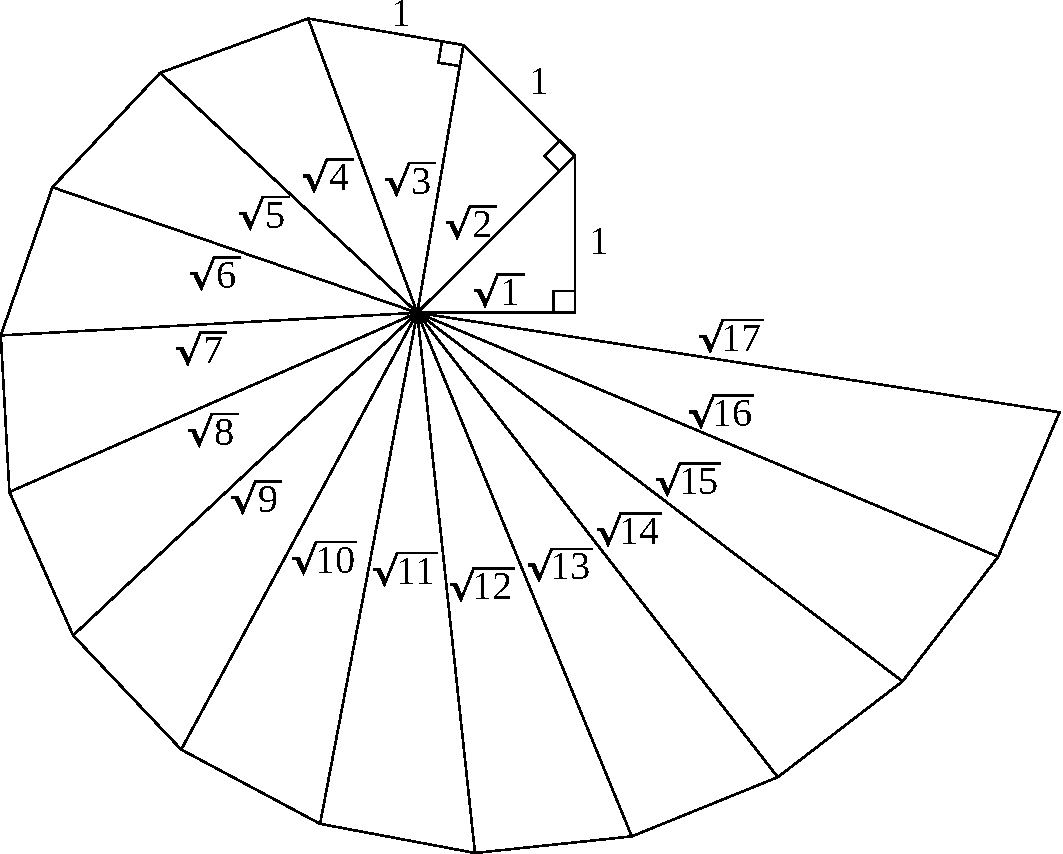
\includegraphics[width=2in]{EPS/Spiral_of_Theodorus-v1.pdf}
%\Caption{\label{fig:TheodorusSpiral}
% Ths ref is resolved on page 33 for Fig 2.1
%\green
The spiral of Theodorus, made from contiguous right triangles having
lengths $a=1$, $b_n=\sqrt{n}$, with $n\in\N$, and $c_n=\sqrt{n+1}$. 
In this way, each value of $c^2_n=b^2_n+a^2\in\N$.
This sequence of triangles generate the set $\{\sqrt{n}\}\in\I$, with $n \in\N$, and is easily generated using a compass and a ruler.
(Adapted from
\texttt{\scriptsize https://en.wikipedia.org/wiki/spiral\_of\_Theodorus}.) \index{spiral of Theodorus} %}
%\end{tcolorbox}
\end{figure}

\paragraph{Public-key security:}
 %\marginpar{\tiny \red Is this the best place for this discussion?} BART
% Briefly describe how public-key systems work
\index{primes} \index{internet security} \index{cryptography} \index{public-key, see cryptography} 
Security is a key application for integers, due to their absolute precision.
Most people assume encryption is best done by a personal login and passwords.
But passwords are fundamentally insecure because it is relatively easy for a computer to search all possible combinations of a computer's keyboard characters
 (including those which use the Shift, CapsLock, Ctrl, Alt, Esc and Windows keys).
 For example the key ``c'' can be modified to be Shift-c, Ctrl-c, Alt-c, Esc-c, etc.

\comment  {\red
Unfortunately the word entropy has a serious flaw since it has two different meanings, first in Claude Shannon's \emph{theory of information}, and second in the \emph{thermodynamics of theory of heat}.
While not iddeal, the different meanings can typically be decoded from the sentence context.
 }

In the field of computer security there is an important concept known as \emph{entropy}.
Unfortunatly the word has two quite different meanings.
One meaning is used in the theory of information, known as \emph{Shannon entropy}, which is a measure of randomnes.
The second meaning is heat \emph{entropy}, a measure of the flow of heat \citep{Allen94a,Allen96f}. 
%  (\S\ref{entropyH}, p.\pageref{entropyH}).
\label{entropyH} \index{entropyH}
\label{entropyS} \index{entropyS}
A bit of Shannon entropy one of two possible outcomes given the flip of a coin.
%Your first guess would be correct half the time, and your second (the other guess) would be correct.
The Shannon entropy for 10 bits is $2^{10} \approx 10^3$ outcomes.
An exhaustive search of 1000 outcomes is trival. 
Twenty bits is $2^{20} \approx 10^6$ possibilities, much harder to guess, but still easily searched.
The realm of 100 bits is $1.27\!\times\! 10^{30}$ possibilities.
% In these example the radix of the numbers is 10.


An important application of prime numbers is public-key  encryption, which is essential for internet security applications (e.g., online banking). % A secure internet is dependent on public-key encryption.
 % \footnote{One might say this as either:
 %   i) a key application of primes, or
 %  ii) it is primary application of keys. (Its a joke.)}
Decryption depends on factoring large integers formed from products of primes having thousands of bits.%
 %BART\footnote{\magenta As a simple but concrete example, a public-key encryption that would be much more secure.
The product of many primes could be the public-key while one large prime, or better, the product of a subset of primes,
 Start with two (or more) primes, such as 5*3 and 5*11, and then using the Euclidean (GCD) algorithm
  %\cite{\ref{Lec 5}}
 to find the common prime, would serve as the private key.
Given the great difficulity in factoring numers into their primes, this can serve as a ``trap-door'' function, since multiplying primes is easy but factoring them can be expensive.  }

 \index{GCD: see greatest common divisor}
 \index{greatest common divisor}
 %Given the difficulty of factoring the numbers into their primes, and ease of finding the GCD using
 %Euclidean algorithm, a practical scheme may be possible.
 % One problem with this idea is that one may store all the known primes.

The security is based on the relative ease of multiplying large primes along with the virtual impossibility of factoring them.
One possible approach is to use the properties of roots of polynomials and Newton's method \citep{Allen24} to generate a key could be useful.

 \index{trap-door function}
A \emph{trap-door function} is one where a computation is easy in one direction but its inverse is very difficult. 
As an example think of a very long list of numbered (indexed) items. If I give you the index, you can look up the item quickly. But if I give you the item as a randomized set of characters, it would be hard (but not impossible) to find the index of the item.
You might start by sorting on the list, which could be difficult.
Consider the problem of sorting all the molecules in 1 liter of a mixture of several gases.
  %The concept follows from large entropy. This complexity (high entropy) is what creates the trap-door.
  % We shall explore trap-door functions in Appendix \ref{Chap:NS}.
  
Public-key encryption is based on a trap-door function. % (p.~\citep{ref.142857}).
If everyone were to switch from passwords to public-key encryption,
the internet would be much more secure.%
 %BART\footnote{\scriptsize \url{https://fas.org/irp/agency/dod/jason/cyber.pdf}} 
\index{internet security} \index{passwords} \index{public-key security}

\BEx
Consider the following method of generating a trap door: The private key is an irrational number \texttt{PRIV} (for example: $\pi, \pi^\pi, \log_\pi(\sqrt{\pi_{101}})$.
The public key \texttt{PUBL} is then a sequence of say 10 integers generated from \texttt{PRIV} using the CFA (see problem \#8 of NS-2, page \pageref{sect:cont_frac}).

How would you propose to recover \texttt{PRIV} given \texttt{PUBL}?

\sol{In my view this is impossible because the space of irrational numbers is more than huge. Knowing the first 10 CFA integers tells you nothing about \texttt{PRIV}.

It is likely that NSA would not accepted such a scheme because it is ``too good.'' It is known that the NSA requires an encryption method that only the NSA can crack in a fixed amount of time, using the world's most powerful computer. The problem with this view is that the \emph{bad guys} can use their own scheme rather than the RSA method.}
\EEx

 \paragraph{Puzzles:}
\label{puzzle}
Another application of integers is imaginative problems that use integers. An example is the classic
Chinese \emph{four stone problem:}
Find the weights of four stones that can be used with a scale to weigh anything (e.g., salt, gold) between
0 and 40 grams (Assignment AE-2, Problem \#5)  %, p.~\pageref{fig:scale})
% renders wrong page #: page \pageref{fig:scale}).
%This ref is correct, but the page number is wrong.
%(Assignment \citep{AE2}, Fig.~\ref{fig:scale}, p.~\pageref{fig:scale}  
% fig:scale is in text; fig:scale-AE2 in sol
The answer is not as interesting as the method, since the problem may be easily recast into a related one.
 %\footnote{Hint: the first two stones have weight of 1 and 3.}
This type of problem can be found in airline magazines as amusement on a long flight. This puzzle is best
cast as a linear algebra problem with integer solutions. Again, once you know the trick, it is ``easy.''%
%\Marginpar{\hspace{2cm}\red\large Verify} BART
 \footnote{Whenever someone tells you something is ``easy,'' you should immediately appreciate that
 it is very hard, but once you learn a basic concept, the difficulty evaporates.}
\index{Chinese four stone problem: see puzzles} \index{puzzles}

%\clearpage %Optional newpage

%\comment
	{% NS-1
\newpage
 \renewcommand{\sol}[1]{} %suppress solution
\index{Homework, see \emph{Assignments}}
\index{Assignments: NS-1}

%\setcounter{scratch}{\value{equation}} %save counter equation in scratch

%%%Dates:
%493 AdvEngMath F22 Aug 22 - Dec 7, 2022
%298CSA S22: March 21 - May 4, 2022
% Update of HW
%% Exam I Lec 12, Apr 15, 2022
%% Exam II 


\newpage

%%%% Modify HW number %%%%%%%%%%
%\newcommand{\HW}{NS \#1 \hfill \date}
%%%%%%%%%%%%%%%%%%%%%%%%%%%%%%%%
%\subsection{Problem NS 1 \hfill \today{\date}}
%\subsection[EXERCISES NS \#1]{Problems: NS \#1}

%{\bf EXERCISES NS-1}
\noindent
\underline{\hspace{\textwidth}}
\section{Problems NS-1}%BART \label{NS1}
\noindent \underline{\hspace{\textwidth}}
 \index{NS-1}


%\noindent \underline{\hspace{0.9\textwidth}}
%\subsection[EXERCISES NS-1]{\bf \large EXERCISES NS \#1}
%{\bf EXERCISES NS-1}
%\noindent\underline{\hspace{0.9\textwidth}}

\noindent \\   %not sure why this \\ is needed
\subsection*{Topic of this homework:}
Introduction to Matlab/Octave (see the Matlab or Octave tutorial for help)

%{\blue Items in blue represent corrections.}
Deliverables: Report with charts and answers to questions.
% Hint: Use \LaTeX.%
%\footnote{ \url{https://www.overleaf.com} }

%%%%%%%%%%%%%%%%%%%%%%%%%%%%%%%%%%%%%%%%%%%%%%%%%%%%%%%%%%%%%%%%%%%%%
% start of problems
%%%%%%%%%%%%%%%%%%%%%%%%%%%%%%%%%%%%%%%%%%%%%%%%%%%%%%%%%%%%%%%%%%%%%

%%%%%%%%%%%%%%%%%%%%%%%%%%%%%%%%%%%%%%%%%%%%%%%%%%%%%%%%%%%%%%%%%%%%%

%Move to Introduction.tex
%\setcounter{problem}{0}
%\setcounter{equation}{0}
%\renewcommand{\theequation}{NS-1 \thechapter.\arabic{equation}}

%%% IMPORTANT %%%
%%% don't use ./input{NS1/NS1} or LaTeX will crash due to recursive overflow
%%%
%%% Indivudual files must be cited so that the Manual.tex and Exams.tex can prune the problems
%%%

%BART\input{./NS1/plot_complex_quantities}
%BART\input{./NS1/course_related}

%%% END %%%

%\setcounter{equation}{\value{scratch}} %restore scratch to equation

\newpage
\renewcommand{\sol}[1]{ {\\blue{\bf Solution:~}#1}{\gray\tiny$\blacksquare$} }
	}%\comment


\section[The role of physics in mathematics]
	{The role of physics in mathematics \label{Lec 3}}
%{\magenta Physics: eigenmodes, bells, music\\ Mathematics: The fundamental theorems }

%\paragraph{Bells, chimes and eigenmodes:}
\index{music}
Integers arose naturally in art, music, and science. Examples include the relationships between musical notes,
the natural eigenmodes (tones) of strings and other musical instruments.  These relationships were so common
that Pythagoras believed that to explain the physical world (the universe), one needed
to understand integers.  As discussed on \S\ref{Chap:IN} (p.~\pageref{Chap:IN}) ``all is number'' was a seductive song.

As we will discuss on page ~\pageref{Lec 10},
it is best to view the relationships among acoustics, music, and mathematics as historical, since these
topics inspired the development of mathematics.  Today integers play a key role in quantum mechanics,
again based on eigenmodes, but in this case, eigenmodes follow from solutions of the Schr\"odinger equation,
with the roots of the characteristic equation being purely imaginary numbers $\in\N$.  If there were a real part (i.e.,
damping), the modes would not be integers. 

%\Marginpar{Put Sch Eq problem from\\ 537 HW in new-VC2.}
 { %\blue
As discussed by Vincent \citet[p.~201]{Salmon46a}, Schr\"odinger's equation follows directly from the Webster
horn equation. While Philip \citet[p.~281]{Morse48} (a student of Arnold Sommerfeld) fails to make the direct link, he comes close to the same
view when he shows that the real part of the horn resistance goes exactly to zero below a cutoff frequency.
 %\Marginpar{\hspace{2cm}Fig 5.3, p.~256} BART
He also discusses the trapped modes inside musical instruments created by the horn flare.
One may assume Morse read Salmon's paper on horns, since he cites Salmon
 \citep[footnote 1, p.~271]{Morse48}.
 %\Marginpar{\red Discuss Sturm-Liouville vs WHEN in new-VC2.\\ \& Discuss \emph{companion matrix} approach.}  BART
 }
 \index{Schr\"odinger's equation}
 \index{Salmon, Vince}
 \index{eigenmodes}
 \index{Schr\"odinger, Erwin}
 \index{quantum mechanics}

Engineers are so accustomed to working with real (vs.~complex) numbers that they rarely acknowledge the distinction between real
(i.e.,  irrational) and fractional numbers.  Integers arise in many
contexts.  One cannot master computer programming without understanding integer, hexadecimal, octal, and
binary representations, since all numbers in a computer are represented in numerical computations in
terms of rationals ($\Q = \Z\cup \F$).
% \footnote{See Appendix \ref{Apdx:Notation} (p.~\pageref{Apdx:Notation}) for a review of mathematical notation.}

The primary reason integers are so important is their absolute precision.  Every integer $n\in \Z$ is unique%
 %BART \footnote{Check out the history of $1729 = 1^3+ 12^3 = 9^3 + 10^3$.
 %GW Hardy and S Ramanujan and story about 1729 and how it fits Pygath Thm two ways
 %Does this violate Euclid's formula? \red Namely, given $c$, when are $a$ and $b$ unique?
 	%}
and has the indexing property, which is essential for making lists that are ordered, so that
one can quickly look things up.  The alphabet also has this property (e.g., a book's index).
 %Other than for hexadecimal numbers, which for notional reasons use the alphabet, other than the base,
 %letters (base 26), are equivalent to integers (base 10) (i.e., they are just as precise).
 %A sequence of letters is equivalent to a sequence of integers.

Because of the integer's absolute precision, the digital computer quickly overtook the analog computer
once it was practical to make logic circuits that were fast.
 %\marginpar{\red \tiny Org?}
From 1946 the first digital computer was thought to be the University of Pennsylvania's ENIAC.
We now know that the code-breaking effort in Bletchley Park, England, under the guidance of Alan Turing,
created the first digital computer (the Colossus), which was used to break the World War II German Enigma code. 
Due to the high secrecy of this war effort, the credit was acknowledged only in the 1970s when the project
was finally declassified.
\index{classification: number theory}

There is zero possibility of analog computing displacing digital computing because of the importance of
precision (and speed).  But even with binary representation, there is a nonzero probability of
error---for  example, on a hard-drive---due to physical noise. To deal with this, error-correcting codes have been
developed, reducing the error by many orders of magnitude. Today error correction is a science,
and billions of dollars are invested to increase the density of bits per area to increasingly
larger factors.  A few years ago the terabyte drive was unheard of; today it is standard. In a
few years petabyte drives will certainly become available.  It is hard to comprehend how these will
be used by individuals, yet they are essential for online (cloud) computing.


\subsection {The three streams of mathematics}
Modern mathematics is built on a hierarchical construct of fundamental theorems, as summarized in the following boxed material  on page \pageref{box:FundamentalThms}.
The importance of such theorems cannot be overemphasized.

Gauss's and Stokes's laws play a major role in understanding and manipulating Maxwell's equations.
Every
engineering student needs to fully appreciate the significance of these key theorems. If necessary, memorize them.
But memorization will not do over the long run, as each and every theorem must be fully understood.
Fortunately most students already know several of these theorems, but perhaps not by name.  In such cases, it is a matter of mastering the vocabulary.

%\begin{table}[ht]
\begin{center}
\footnotesize
\begin{minipage}{.65\textwidth}
\begin{tcolorbox}
{\bf \large The three streams of mathematics}
%\Caption{
\label{box:FundamentalThms}
%The fundamental theorems of mathematics.
% See \citet{Flanders80} for a discussion on integration under the integral sign, relevant for stream 3.
%	}%\caption
%\noindent\rule{\textwidth}{0.2pt}
 \Be %{
\item {\bf Number systems: Stream 1}
	\Bi
\item Arithmetic
\item Prime numbers
	\Ei
\item {\bf Geometry: Stream 2}
	\Bi
\item Algebra
%\item B\'ezout
	\Ei
\item {\bf Calculus: Stream 3}
\citep{Flanders80}
% \footnote{Flanders, Harley (June--July 1973). ``Differentiation under the integral sign.''
%  \emph{American Mathematical Monthly} 80 (6): 615-627. doi:10.2307/2319163. JSTOR 2319163.}
	\Bi
\item Leibniz $\R^1$
\item Complex $\C \subset \R^2$
\item Vectors $\R^3, \R^n, \R^\infty$
 \Bi
\item Gauss's law (divergence theorem)
\item Stokes's law (curl theorem, or Green's theorem)
\item Vector calculus (Helmholtz's decomposition theorem)  % (FTVC))
 \Ei
\index{Helmholtz's decomposition theorem}
	\Ei
\Ee %}
%\noindent\rule{\textwidth}{0.2pt}
\end{tcolorbox}
\end{minipage}
\end{center}
%\end{table}


%Review of all the FT
%  \Bi
%\item Arithmetic
%\item Prime number theorem
%\item Algebra
%\item Cauchy's theorem
%\item Calculus (e.g., Leibniz $\R^1$, Complex $\C, \R^2$, Vector $\R^n$)
%\item Green's (e.g., Gauss'. and Stokes's) theorems%
%  \Ei

The fundamental theorems are naturally organized and may be thought of in terms of the three streams of \citet{JS10}.
 %
For Stream 1 we have the fundamental theorem of arithmetic and the prime number theorem. 
\index{prime number theorem}
\index{stream 1}
 %
For Stream 2 there is the fundamental theorem of algebra,% and B\'ezout's theorem,
\index{stream 2}
and for Stream 3 there are a host of theorems on calculus, ordered by their dimensionality. 
\index{stream 3}
Some of these theorems seem trivial (e.g., the fundamental theorem of arithmetic).  Others are
more challenging, such as the fundamental theorem of vector calculus and Green's theorem.

Complexity should not be confused with importance. Each of these three theorems, as stated, is fundamental.
Taken as a whole, they are a powerful way of summarizing mathematics.


\begin{figure}[htb]
% pwd /home/BACKUP/usr/UIUC/Springer/SubmitSpringer.24/M/PrimeRatio.m
%matlab: PrimeRatio.m
 %
\centering
%\figure generated with ~/M/PrimeRatio.m using matlab R2019
% The exact values of the red and green curves needs to be computed using LeastSquares on log-log coordinates
 %
% Convert to pdf using 'ps2pdf PrimeRatio.eps'
 %
% \includegraphics[trim={0.cm 0.cm 7.5cm 17.cm},clip,width=5in,height=3in,width=0.95\textwidth] %Orig
% \includegraphics[trim={10.35cm 2.5cm 8.4cm 21.cm},clip,width=5in, height=3in,width=0.95\textwidth] %%GOOD
% \includegraphics[trim={10.35cm 2.5cm 8.4cm 22.cm},clip,width=5in,height=5in,width=0.95\textwidth] %Very GOOD
% \includegraphics[trim={0.9cm 0.cm 3.9cm 14.5cm},clip,width=5in,height=3in,width=0.95\textwidth] %Orig
 % spit out the graphic
 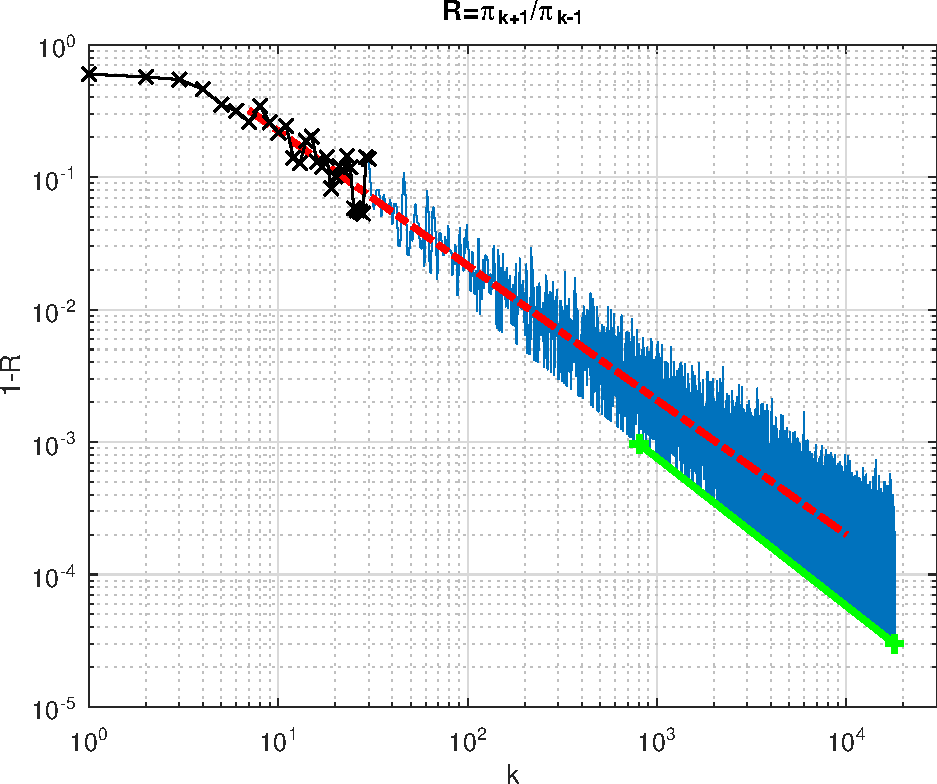
\includegraphics[trim={0cm 0cm 0cm 0cm},clip,width=5in,height=4in,width=0.95\textwidth]{./M/PrimeRatio.eps}
%
%\Caption{ \label{fig:PrimeRatio}
This figure succinctly summarizes all of the known theorems that are know about prime numbers, in one
	simple graph, as a log-log plot of $|1-R_k|$.
Here $R_k$ is defined as
 $\pi_{k+1}/\pi_{k-1}>1 \underset{k\rightarrow \infty}{\rightarrow} 1$.
 %%% \purple $1\!-\!R_k = (\pi_{k-1}-{\pi_{k+1}})/{\pi_{k-1}}$ as $k \rightarrow \infty$. \black
%
 Thus $R_k$ has the strange property that it is a random varliable, always greater than 1,
	with a standard deviation $\sigma_{_R}>0$.
However, in the limit of large $k$, since $R_k$ goes exactly to 1, $|1-R_k| \rightarrow 0$.
%
\purple
In brief, since each prime is larger than it predecessor, $R_k>1 \rightarrow 1$, yet,
	in the limit, $|1-R_k|  \underset{k\rightarrow \infty}{\rightarrow} 0.
	$
%
\red
	How this shows up in the chart is interesting.
\black
%
Note that since $R_k$ is a random variable, one must estimate both the mean and standard deviation, which is a decreasing function of $k$.
However $|1-R| = |R-1|>1 \rightarrow 0$ as $k \rightarrow \infty$.
 %
From the chart, the difference $|1\!-\!R_k|$ appears to be close to linear on a log-log scale (red dashed line)
	\citep[p.~9, 5$^{th}$ Edition]{HardyWright38}.
The function $1\!-\!R_k$ is characterized by the red dashed line, which is $\approx 2.0\!\times\! 10^{-4}$ for $k=1e4$.
	{\brown
	Note how the {\cyan cyan} line on the lower bound of the data, defines a straight line, with a linear slope
	(on log-log coordinates), that is slightly steeper than the red-dashed median line.
	For $k\leq30$, the points are labled with an {\black $\times$}.
The upper bound is random.
This well defined lower bound implies a structure in the lower bound of $R(k)$, which requires further study
	{(\sc ./M/PrimeRatio.eps)}.
	}
	}
\end{figure}


%%%%%%%%%%%%%%%%%% STREAM 1 Fund Thms %%%%%%%%%%%%%%%%%%
%{\magenta Discussion of fundamental theorem of arithmetic \& prime number theorem}
\subsection{Stream 1: Prime number theorems \label{FT:PN}}
\index{stream 1}
\index{fundamental theorem: prime numbers}
\index{primes}
There are two key fundamental theorems is
\Be
\label{FT:AR}
\index{fundamental theorems: arithmetic}
\item \emph{The fundamental theorem of arithmetic}:
The first and best know theorem is that every integer $n\in \Z$ may be uniquely factored into prime
numbers.
A prime number has no factors other than 1 and itself.
For example, prime factors of 6 are 2 and 3 since $6=2\times 3$. 
The product of two integers $m,n\in\Z$ is $mn=\sum_m n = \sum_n m$. For example, $2\times3 = 2+2+2 = 3+3$.
The two cases give the same result, thus we may decide which we prefer.
There is no \emph{a priori} answer without more information.

For example, if the two numbers are $m=1000$ and $n=10$, should we add $m$ 10 times or $n$ 1000 times?
This is difficult to establish without more information.
It requires the definition of how the sums are to be computed.

An interesting example is $93,235,723\times2$.
I suspect the answer is obvious in this example.
My veiw is that 93235723 + 93235723 is easier that $(2+2+2 \cdots +2)\times93235723$.
The only way to find out is to actually time the computation using what ever method you choose to use.
Obvious choices are:
1) use pencil and paper,
2) work on a hand calculator,
3) on a personal computer,
4) an abacus, or
5) give the problem to a friend to work out.
When working on a computer in Matlab/Octave, if the data is saved in a $n,m$ matrix, a modern
computer will use vectorized algebra, making the calculation in near real-time.
The limit is then determined by the memory of the cpu and the system's arithmetic vectorized
coprocessor (GPU) for numeric calculations.

It may be important to note the factors of $93,235,723 = 7 \times 317 \times 42,017$.

 \index{PNT: prime number theorem}
\item \emph{The prime number theorem:}
One would like to know how many primes there are. That is easy: $|\P|=\infty$  (the
size of the set of primes is infinite).  A better way of asking this question is
What is the average density of primes in the limit as $n \rightarrow \infty$?
This question was answered, for all practical purposes, by Gauss, who in his free time computed
the first three million primes by hand. He discovered that, to a good approximation,
the primes are equally likely on a log scale. This is nicely summarized by the couplet:
%aka: Bertrand's conjecture (Paris, 1845)
 \begin{quote}
% {\sl
Chebyshev said, and I say it again: There is always a prime between \emph{n} and \emph{2n}.
% }%\sl
\label{FT:PNT}
 \end{quote}
 
This alludes to the mathematician Pafnuty Chebyshev, who proved the prime number theorem in a novel way
\citep[p.~585]{JS10}.
 \index{Chebyshev} \index{prime number theorem}

When the ratio of two frequencies (pitches) is 2, the relationship is called an \emph{octave}.
With a slight stretch of terminology, we could say there is at least one prime per octave.
\index{octave}
\Ee

%

\BEx
An interesting extension of Chebyshev's observation might be the density in primes per fraction of an octave?
An alternative is to study the ratio $\pi_{k+1}/\pi_{k-1} <1$ as $k \rightarrow \infty$, or perhaps $\log_2 \pi_{n+1}/\pi_{n-1}$.

\sol{An answer is suggested by Fig.~\ref{fig:PrimeRatio}, showing a log-log plot of $1-R_k$.
Note that the graph has a well defined lower bound, having a slope slightly steeper than the red dashed line.
 }
\EEx

In modern western music the octave is further divided into 12 ratios called \emph{semitones}, equal to
$\sqrt[12]{2}$. Twelve semitones is an octave.  In the end, it is a question of the density of primes
on a log-log (i.e., ratio) scale.
Figure \ref{fig:PrimeRatio} is a log-log plot of $R={\pi_{k+1}}/{\pi_{k-1}}$
as a function of $k$, namely a 
plot of $\log_{10}(\pi_{k+1}/\pi_{k+1})$ vs.~$log_{10} k$.
  %
A linear fit to this log-log plot requires two points to determine the line.
The equation for this line may be computed by fitting two points.
%Taking the first is at $k=10$ where $1-R(10)\approx 0.2$, and the second at $k\approx 0.8\times10^{4}$, then $1-R({8\! \times\!10^{5}}) \approx 5.8\!\times \! 10^{-5}$.
%	Thus $R(8\!\times\! 10{^{-5}}) \approx 6.0\times 10^{-5}$.
% }
%%\newline {\red Scale the red dashed line up by 2x to fit the mean of the random curve on the log-log scale.} 
%{\violet \it \tiny \bf Verified Apr 19, 2024}

One might wonder about the maximum number of primes per octave in the neighborhood of $N$, or ask for the
fractions of an octave (factors of 2) for $\pi_k$ as $k$ becomes large.
The maximum value of $R_k<0.5$; thus Chebyshev's bound of 2 is conservative.

As $k\rightarrow \infty$ the bound is exponentially compressed.  The results of this
calculation are shown in Fig.~\ref{fig:PrimeRatio}. 
For reference, when $k=10$, $\pi_{9}/\pi_{11} = 0.741935483870968$,
thus $1-R(11)/R(9) = -0.347826086956522$.
When $k=9580$, $1-R_k \approx 2.0043\!\times\! 10^{4}$.

It is an important observation that the reciprocals of prime numbers are rational
 %\Marginpar{Possible HW problem.} BART

 Note that by trial and error, it is quick and easy to find the first prime below any number.
 Within 5 tries one will typically find a prime.
 Most primes have a small prime factor \{3, 4, 5, 7, 11, 13\}.
 By trial and error, start with the small primes and you will quickly find a factor.
 Exceptions are rare, which is why primes are hard to search for. They have no small factors

 An alternative is to use the octave command $P=primes(1e4)$, which gives large primes, such as
 $P(1229)=9973$.
To verify: $factor(9969)=[3,3323]$ or $factor(1745) = [5,349].$
 Using $P=primes(2e4)$ then $P(2262)=19997$, and $factor(19995)= [3, 5, 31, 43]$.
%BART\footnote{\olive We may fit a straight line on this figure to estimate the slop of the minimum
%points, thus giving a numberical slope to the curve.  I suspect the answer will reveal a simple
%formula for $R(k)$. 
% }
  %red, green, blue, cyan, magenta, yellow, black, gray, white, darkgray, lightgray, brown, lime, olive,
  % orange, pink, purple, teal, violet.


%%%%%%%%%%%%%%%%%% STREAM 2 Fund Thms %%%%%%%%%%%%%%%%%%
\subsection{Stream 2: Fundamental theorem of algebra \label{FT:AE}}
 \index{fundamental theorem: algebra}
This theorem states that every polynomial in $x$ of degree $N$,
\be
P_N(x) = \sum_{k=0}^N a_k x^k,
\ee
has at least one root (see p.~\pageref{Lec 12}).
When a common root is factored out, the degree of the polynomial is reduced by 1.
Applied recursively, a polynomial of degree $N$ has $N$ roots. Note there are $N+1$ coefficients
(i.e., $[a_N, a_{N-1}, \dots, a_0]$).  If we are interested only in the roots of $P_N(x)$, it is best
to define $a_N=1$, which defines the monic polynomial.  If the roots are fractional numbers ($\in\F$), this
might be possible. However, when the roots are irrational numbers (likely), a perfect factorization is
at least unlikely, if not impossible.
\index{stream 2} \index{composition} \index{monic polynomial}
The best we can do seems to be a search for fractional roots $s_k \in\F$ that minimize the norm of $P_N$
\be
 \min_{s_k}||P_n|| = \min_{s_k} |P_N(\widehat{a}_k,\widehat{s}_k)|.
\ee


%%%%%%%%%%%%%%%%%% STREAM 3 Fund Thms %%%%%%%%%%%%%%%%%%
\subsection{Stream 3: Fundamental theorems of calculus \label{FT:SVC}}
\index{stream 3}
 %{\magenta Discuss FTs of integration: $\R, \C, \R^3$, e.g., Green's Thms, Helmholtz Thm of Vector Calculus}

In \S \ref{Lec 39:GSLaw} and \S\ref{Lec 40} we will deal with each of the theorems for Stream 3. We consider the several fundamental theorems of integration, starting with Leibniz's
formula for integration on the real line ($\R$), then progressing to complex integration in the
complex plane ($\C$) (Cauchy's theorem), which is required for computing the inverse Laplace
transform. Gauss's and Stokes's laws for $\R^2$ require closed and open surfaces, respectively.
One cannot manipulate Maxwell's equations, fluid flow, or acoustics without understanding these theorems.
Any problem that deals with the wave equation in more than one dimension requires an understanding of
these theorems. They are the basis of the derivation of the Kirchhoff voltage and current laws, as first proposed by Newton for mechanics
and acoustics.
 % \index{Laplace transform} \index{Leibniz}%\index{Green} \index{Helmholtz}
\index{Cauchy, Augustin-Louis}
\index{Gauss, Carl Friedrich}
\index{Stokes, George}
\index{Maxwell, James}
\index{Kirchhoff, Gustav}

\index{$\Laplacian()$: see Laplacian}
 %\subsubsection[Integration is 2 and 3 dimensions]{The fundamental theorem of vector calculus}
Finally we define three vector operations based on the gradient operator,
%differential vector operator, which have been given mnemonic abbreviations (see p.~\pageref{Lec 40}),
\be
\Grad \equiv
 \i \frac{\partial}{\partial x} + \j \frac{\partial}{\partial y} + \k \frac{\partial}{\partial z},
\label{eq:Grad1}
\ee
 pronounced as either ``del'' or ``nabla,'' which are the
  gradient $\Grad()$,
  divergence $\Div()$,
  wedge $()\!\wedge\!()$
  and
  curl $\Curl()$.

Second-order operators such as the 
 scalar Laplacian $\Div\Grad() = \Grad^2()$, the divergence of the gradient (\DoG), may be constructed
 from first-order operators. The most important of these is the vector Laplacian $\VectorLaplacian()$,
the gradient of the divergence (\gOd) which is required when working with Maxwell's
wave equations.%
 %BART\footnote{See \S \ref{Lec 40} (p.~\pageref{Lec 40}) for the definitions of \DoG\ and \gOd.}

The first three operations are defined in terms of integral operations on a surface in one, two, or three dimensions
by taking the limit as that surface, or the volume contained within, goes to zero.  These three differential operators are essential to fully understand Maxwell's equations, the crown jewel
of mathematical physics.  Hence mathematics plays a key role in physics, as does physics in math.
 \index{gradient $\Grad()$} \index{divergence $\Div()$} \index{curl $\Curl()$}
 \index{Laplacian, scalar: $\Grad^2$} \index{Laplacian, vector $\VectorLaplacian$}
 \index{Maxwell's equations}

\subsection {Other key mathematical theorems}
 %Table \ref{box:FundamentalThms} item 2 identifies several Other key concepts. %incrementally Remove table
In addition to the widely recognized fundamental theorems,
there are a number of equally important theorems that have not yet been labeled ``fundamental.''%
 %BART\footnote{It is not clear what it takes to reach this more official sounding category.}
 \index{fundamental theorem: calculus (Leibniz)}
 \index{fundamental theorem: complex calculus (Cauchy)}
 \index{fundamental theorem: vector calculus (Helmholtz)}
 \index{fundamental theorem: arithmetic}
 \index{fundamental theorem: algebra}

 \index{Cauchy's integral theorem}
 \index{complex frequency}
The widely recognized Cauchy integral theorem is an excellent example, since it is a steppingstone
to Green's theorem and the fundamental theorem of complex calculus.
In \S \ref{Lec 27} (see p.~\pageref{Lec 27})		 %Chapter \ref{Chap:SC}
we clarify the contributions of each of these special theorems.  
\index{stream 3}
\index{stream 2}

Once these fundamental theorems of integration (Stream 3) have been mastered, the student is ready
for the complex frequency domain, which takes us back to Stream 2 and the
complex frequency plane ($s= \sigma+\omega\jmath \in \C$). 
While the Fourier and and Laplace transforms are taught in mathematics courses, the concept of complex
frequency is rarely mentioned.
The complex frequency domain (see p.~\pageref{LaplaceFrequency}) and causality are
fundamentally related (see pp.~\pageref{Lec 28}--\pageref{Lec 30}),
and are critical for the analysis of signals and systems, especially when dealing with the concept
of impedance (see p.~\pageref{Lec 25}).

Without the concepts of time and frequency we cannot develop an intuition for the Fourier and Laplace
transforms, especially within the context of engineering and mathematical physics.
The Fourier transform covers signals, while the Laplace transform \LT\ describes systems. Separating these
two concepts, based on their representations as Fourier and Laplace transforms, is an important
starting place for understanding physics and the role of mathematics. However, these methods, by
themselves, do not provide the insight into physical systems that we need to be productive or, better,
creative with these tools. We need to master the tools of differential equations and then partial
differential equations to fully appreciate the world that they describe. Electrical 
networks composed of inductors, capacitors, and resistors are isomorphic to mechanical systems
composed of masses, springs, and dashpots. Newton's laws are analogous to those of Kirchhoff,
which are the rules needed to analyze simple physical systems composed of linear (and nonlinear)
subcomponents. When lumped-element systems are taken to the limit in several dimensions, we obtain
Maxwell's partial differential equations, the laws of continuum mechanics, and beyond.

The ultimate goal of this text is to make you aware of and productive in using these tools.
This material can be best absorbed by treating it chronologically through history, so you
can see how this body of knowledge came into existence, through the minds and hands of Galileo,
Newton, Maxwell, and Einstein. Perhaps one day you too can stand on the shoulders of the giants who
went before you.

\section {Applications of prime numbers \label{Lec 4}}

If someone asked you for a theory of counting numbers, I suspect you would laugh and start counting.
It sounds like either a stupid question or a bad joke.  Yet integers are a rich topic, so the question
is not even slightly dumb.
 %\footnote{\scriptsize Nice discussion of primes: \url{https://www.quantamagazine.org/mathematicians-discover-prime-conspiracy-20160313/} }
It is somewhat amazing that even birds and bees can count.  While I doubt birds and bees can recognize
primes, cicadas and other insects crawl out of the ground only in prime-number cycles (e.g., 13- or
17-year cycles). If you have ever witnessed such an event (I have), you will never forget it. 
Somehow they know.  Finally, there is the Euler zeta function, first introduced by Euler based on his
analysis of sieve of Eratosthenes, now known as the Riemann zeta function $\zeta(s)$, that is
\emph{complex--analytic}, with its poles at the logs of the prime numbers. 
The properties of this function are truly amazing, even fun.
Many of the questions and answers about primes go back to at least the early Asian
mathematicians (ca.~1500 BCE).

%The exact relationship between the primes and the poles will be discussed on p.~\pageref{AE1}.
 % \footnote{The Riemann zeta function is known as the million dollar equation as there is a cash
 %  reward for a proof of the Riemann Hypothesis.}
\index{Riemann zeta function}
 \index{zeta function, Euler} \index{$\zeta(x)$, Euler zeta function}
 \index{zeta function, Riemann} \index{$\zeta(s)$, Riemann zeta function}

%%%%%%%%%%%%%%%%%%%%%%%%%%%%%%%%%%%%%%%%%%%%%%%%%%%%%%%%%%%%%%%%%%%%%%%%%%%%%%%%%
\begin{figure}[htbp]

 \begin{tcolorbox}
The recursive ``sieve'' method for finding primes was first devised by the Greek Eratosthenes
 \citep{o2009genuine}.
 \end{tcolorbox}
\vspace*{1cm}

	\Be %2
\item Write $N-1$ integers $n$, starting from $2$: $n \in \{2, 3, \dots, N\}$
 (e.g., $N=4, n \in \{2, 3, 4\}$).  Note that the first element $\pi_1=2$ is the first prime.
 Cross out all multiples of $\pi_1$; that is, cross out $n\cdot\pi_1 = {\red, 6, 8, 10, \dots, 50}$,
 or all $n$ such that \texttt{mod(n,$\pi_1$)}= 0.
 \begin{tcolorbox}
 \begin{center}
\begin{tabular}{r r r r r r r r r r}
     & {\bf \red 2} & 3 & $\cancel{\ 4}$ & 5 & $\cancel{\ 6}$ & 7 & $\cancel{\ 8}$ & 9 & $\cancel{10}$ \\
  11 & $\cancel{12}$ & 13 & $\cancel{14}$ & 15 & $\cancel{16}$ & 17 & $\cancel{18}$ & 19 & $\cancel{20}$ \\
  21 & $\cancel{22}$ & 23 & $\cancel{24}$ & 25 & $\cancel{26}$ & 27 & $\cancel{28}$ & 29 & $\cancel{30}$ \\
  31 & $\cancel{32}$ & 33 & $\cancel{34}$ & 35 & $\cancel{36}$ & 37 & $\cancel{38}$ & 39 & $\cancel{40}$ \\
  41 & $\cancel{42}$ & 43 & $\cancel{44}$ & 45 & $\cancel{46}$ & 47 & $\cancel{48}$ & 49 & $\cancel{50}$ \\
\end{tabular}
 \end{center}
 \end{tcolorbox}

\item Let $k=2$ and note that $\pi_2=3$. 
 Cross out $n\pi_2 \; 3\cdot({\red, 3, 4, 5, 6, 7, \dots, 45})$, that is, all $n$ such that \texttt{mod(n,$\pi_2$)}= 0.
 \begin{tcolorbox}
 \begin{center}
\begin{tabular}{r r r r r r r r r r}
     & {\bf \red 2} & {\bf \red 3} & $\cancel{\ 4}$ & 5 & $\cancel{6}$ & 7 & $\cancel{\ 8}$ & $\cancel{\red\ 9}$ & $\cancel{10}$ \\
11 & $\cancel{12}$ & 13 & $\cancel{14}$ & $\cancel{\red 15}$ & $\cancel{16}$ & 17 & $\cancel{18}$ & 19 & $\cancel{20}$ \\
$\cancel{\red 21}$ & $\cancel{22}$ & 23 & $\cancel{24}$ & 25 & $\cancel{26}$ & $\cancel{\red 27}$ & $\cancel{28}$ & 29 & $\cancel{30}$ \\
31 & $\cancel{32}$ & $\cancel{\red 33}$ & $\cancel{34}$ & 35 & $\cancel{36}$ & 37 & $\cancel{38}$ & $\cancel{\red 39}$ & $\cancel{40}$ \\
41 & $\cancel{42}$ & 43 & $\cancel{44}$ & $\cancel{\red 45}$ & $\cancel{46}$ & 47 & $\cancel{48}$ & 49 & $\cancel{50}$ \\
\end{tabular}
 \end{center}
 \end{tcolorbox}


\item Let $k=3, \pi_3=5$. Cross out $n\pi_3 \cdot ({\red 25, 35})$ (\texttt{mod(n,5)=0}).
 \begin{tcolorbox}
 \begin{center}
\begin{tabular}{r r r r r r r r r r}
     & {\bf \red 2} & {\bf \red 3} & $\cancel{\ 4}$ & {\bf\red 5} & $\cancel{\ 6}$ & {\bf\red 7} & $\cancel{\ 8}$ & $\cancel{\ 9}$ & $\cancel{10}$ \\
  {\bf\red 11} & $\cancel{12}$ & {\bf\red 13} & $\cancel{14}$ & $\cancel{15}$ & $\cancel{16}$ & {\bf\red 17} & $\cancel{18}$ & {\bf\red 19} & $\cancel{20}$ \\
  $\cancel{21}$ & $\cancel{22}$ & {\bf\red 23} & $\cancel{24}$ & $\cancel{\red 25}$ & $\cancel{26}$ & $\cancel{27}$ & $\cancel{28}$ & {\bf\red 29} & $\cancel{30}$ \\
  {\bf\red 31} & $\cancel{32}$ & $\cancel{33}$ & $\cancel{34}$ & $\cancel{\red 35}$ & $\cancel{36}$ & {\bf\red 37} & $\cancel{38}$ & $\cancel{39}$ & $\cancel{40}$ \\
  {\bf\red 41} & $\cancel{42}$ & {\bf\red 43} & $\cancel{44}$ & $\cancel{45}$ & $\cancel{46}$ & {\bf\red 47} & $\cancel{48}$ &
$\cancel{49}$ & $\cancel{50}$ \\
\end{tabular}
 \end{center}
 \end{tcolorbox}


\item
 Finally let $k=4, \pi_4=7$ (\texttt{mod(n,7)=0}). Cross out $n\pi_4$: ({49}). 
Thus there are 15 primes less than $N=50$:
$\pi_k=2,3,5,7,11,13,17,19,23,29,31,37,41,43,47$ (highlighted in red). Above 2, all end in odd
numbers, and above $5$, all end with $1, 3, 7,$ or $9$.
	\Ee %2
\vspace{-4mm}
%\Caption{ \label{fig:sieve}
%\index{prime sieve}
\index{Eratosthenes}
Sieve of Eratosthenes for $N=50$.
	}
\end{figure}

%\clearpage

%%%%%%%%%%%%%%%%%%%%%%%%%%%%%%%%%%%%%%%%%%%%%%%%%%%%%%%%%%%%%%%%%%%%%%%%%%%%%%%%%

%\paragraph{Primes $\mathbb P$ \label{sect:NS}}
%\Marginpar{\hspace{1.7cm}ck for accuracy?}

\subsection{The importance of prime numbers}
While each prime perfectly predicts multiples of that prime, but there seems to be no regularity in predicting
primes.
  %themselves explaining irregularities of numbers. 
It follows that prime numbers are the key to the theory of numbers because of the fundamental theorem of arithmetic (FTA).
\index{fundamental theorem: arithmetic}

It is likely that the first insight into the counting numbers started with the sieve shown in Fig.~\ref{fig:sieve}.
A sieve answers the question How can one identify the prime numbers?
The answer comes from looking for irregular patterns in the counting numbers.
 \index{Eratosthenes}
\index{primes, Eratosthenes}
\index{prime sieve}
\index{sieve}

%moved from Intro page 33 Lec 4
%\subsubsection{Sieves} \index{sieve}


 %  \footnote{\scriptsize\url{https://en.wikipedia.org/wiki/Sieve_of_Eratosthenes\#Euler.27s_Sieve} }
%(276-194, {\small BCE}). 
%, and summarized in Fig.~\ref{fig:sieve}.  %Citation to table 2.2. Now commented out 

%For example,
Starting from $\pi_1 = 2$, we strike out all even numbers $2\dot(2, 3, 4, 5, 6, \dots)$ but not $2$. 
Here we use the subscript to count the primes ($\pi_4=7$ and $\pi_5=11$).
By definition,
the multiples are products of the target prime ($2$ in our example) and every other integer ($n\ge 2$).
In this way all the even numbers are removed in this first iteration.  The next remaining integer
($3$ in our example) is identified as the second prime $\pi_2$.  Then all the multiples of $\pi_2=3$
   %(i.e., $\lfloor N/\pi_2\rfloor -1$)
are removed.  The next remaining number is $\pi_3=5$, so all multiples of $\pi_3=5$ are removed
(i.e., $\cancel{10}$, $\cancel{15}$, {$\cancel{25}$}, $\dots$).  This process is repeated until
all the numbers of the list have been either canceled or identified as prime.

As the word \emph{sieve} implies, this process takes a heavy toll on the integers, rapidly pruning
the non-primes.  In four iterations of the sieve algorithm, all the primes less than $N=50$ are identified
in red.  The final set of primes is displayed in step 4 of Fig.~\ref{fig:sieve}.

Once a prime greater than $N/2$ has been identified ($25$ in the example), the recursion stops, since
twice that prime is greater than $N$, the maximum number under consideration.  Thus once $\sqrt{49}$
has been reached, all the primes have been identified (this follows from the fact that the next prime
$\pi_n$ is multiplied by an integer $n = 1, \ldots, N$).
 %Once this number $n \pi_n > N$ the list has been exhausted, since $n < \sqrt{N}$.

When we use a computer, memory efficiency and speed are the main considerations.
There are various schemes for making the sieve more efficient. For example, the recursion $n\pi_k =
(n-1)\pi_k +\pi_k$ will speed up the process by replacing the multiplication with an addition of $\pi_k$.



\subsection{Two fundamental theorems of primes}
Early theories of numbers revealed two fundamental theorems (see \S\ref{FT:AE} and \ref{FT:SVC}). The first of these is
the fundamental theorem of arithmetic, which says that every integer $n\in\N$ greater than 1 may
be uniquely factored into a product of primes:
 \be
n = \overset{K}{\underset{k=1}{\Pi}} \pi_k^{\beta_k},
\label{eq:PrimeFactors}
 \ee
where $k= 1,\ldots,K$ indexes the integer's $K$ prime factors $\pi_k\in\P$.
Typically prime factors appear more than once---for example, $25=5^2$. To make the notation compact
we define the \emph{multiplicity} $\beta_k$ of each prime factor $\pi_k$.  For example,
$2312 = 2^3 \cdot 17^2 = \pi_1^3 \; \pi_7^2 $ (i.e., $ \pi_1=2, \beta_1=3; \pi_7=17, \beta_{7}=2 $) and
$2313 = 3^2 \cdot 257 = \pi_3^2 \; \pi_{55} $ (i.e., $\pi_2=3, \beta_3=2; \pi_{55}=257, \beta_{55}=1$).
 %
Our demonstration of this is empirical, using the Matlab/Octave \texttt{factor(N)} routine, which
factors $N$.%
 %BART\footnote{If you wish to be a mathematician, you need to learn how to prove theorems.  If you're a
%BART physicist, you are happy that someone else has already proved them, so that you can use the result.}

What seems amazing is the unique nature of this theorem.  Each counting number is uniquely
represented as a product of primes. No two integers can share the same factorization.
Once you multiply the factors out, the result is unique ($N$). Note that it's easy to multiply
integers (e.g., primes) but expensive to factor them. And factoring the product of three primes
is significantly more difficult than factoring two.

Factoring is much more expensive than division. This is not due to the higher cost of division
over multiplication, which is less than a factor of 2.%
 %BART\footnote{\scriptsize\url{https://streamcomputing.eu/blog/2012-07-16/how-expensive-is-an-operation-on-a-cpu/}}
Dividing the product of two primes, given one, is trivial, slightly more expensive that multiplying.
Factoring the product of two primes is nearly impossible, as one needs to know what to divide by.
 %This is an explosion in probability, measured by \emph{Shannon entropy}. See more detailed disc below
Factoring means dividing by some integer and obtaining another integer with remainder zero.

This brings us to the prime number theorem (PNT). The security problem is the reason these two theorems are so important:
 (1) Every integer has a unique representation as a product of primes, and
 (2) the density of primes is large (see the discussions on p.~\pageref{FT:PNT}).
Thus security reduces to the ``needle in the haystack problem'' due to the cost of a deep search. 
One could factor a product of primes $N=\pi_k \pi_l$ by doing $M$ divisions, where $M$
is the number of primes less than $\sqrt{N}$. This assumes the primes less than $\sqrt{N}$ are known.
However, most integers are not a simple product of two primes.
Sometimes this is know as \emph{Shannon entropy}.
\label{entropyS}   %(\S\ref{ShannonEntropy}).
\index{Shannon entropy$_S$}
%\index{entropy$_S$}
But the utility of using prime factorization has to do with their density.  If we were simply looking up
a few numbers from a short list of primes, it would be easy to factor them. But given that their density
is logarithmic ($>$1 per octave, as shown in Fig.~\ref{fig:PrimeRatio}), factoring comes at a very high computational cost compared to a table lookup.
 \index{prime number theorem}

\subsection {Greatest common divisor (Euclidean algorithm) \label{Lec 5}} 
\index{GCD}
\index{Euclidean algorithm}
\index{greatest common divisor}

The Euclidean algorithm is a systematic method known to all
educated people, identical to how we perform long division.
The largest common integer factor $k$ between two integers $n$ and $m$ (divisor and dividend) is denoted $k = \gcd(n,m)$,
where $n,m,k \in \N$ \citep{GrahamEtAl94}. 
For example, $15 = \text{gcd}(30, 105)$ since, when factored,
$(30, 105) = (2\cdot 3 \cdot 5, \, 7 \cdot 3 \cdot 5)= 3\cdot 5 \cdot (2,7) = 15\cdot(2, 7)$. 
Thus the GCD is $15$.
Two integers are said to be \emph{coprime} if their GCD is 1
(i.e., they have no common prime factor).
The Euclidean algorithm was known to the Chinese (i.e., not discovered by Euclid) \citep[p.~41]{JS10}.
\index{coprimes}

% BEGIN SLIDE-------------------------------------------------------------------
\begin{figure}[ht]
\begin{tcolorbox}
\centering
%\begin{minipage}{0.95\textwidth}
{\bf \large Examples of the GCD: $l=\gcd(m,n)$}
\footnotesize \setlength{\baselineskip}{.5em} \sl
\emph{
\Bi
\item Examples ($m,n,l\in\Z$):
	\Bi
\item $5=\gcd(13\cdot 5,11\cdot 5)$. The GCD is the common factor 5.
\item $(13\cdot 10,11\cdot 10$) = $10\gcd(130,110) = 10 = 2\cdot 5$ is not prime
\item $\gcd(1234,1024) = 2$, since $1234=2\cdot 617, 1024=2^{10}$
\item $\gcd(\pi_k \pi_m$, $\pi_k \pi_n$) = $\pi_k$
\item $l=\gcd(m,n)$ is the part that cancels in the fraction $m/n \in F$
\item ${m}/{\gcd(m,n)} \in \Z$ 
	\Ei
\item \emph{Coprimes} ($m\perp n$) are numbers that have no distinct common factors; that is,
 $\gcd(m, n) = 1$
 \Bi
\item The GCD of two primes is always 1: $\gcd(13, 11) = 1$, $\gcd(\pi_m,\pi_n) = 1$ ($m\ne n$)
\item $m=7\cdot13, n=5\cdot19 \Rightarrow (7\cdot 13) \perp (5\cdot19)$
\item If $m \perp n$, then $\gcd(m,n)=1$.
\item If $\gcd(m,n)=1$, then $m \perp n$.
 \Ei
\comment
	{% too complex, off topic
\item The GCD may be extended to polynomials--for example, $\gcd(ax^2+bx+c,\, \alpha x^2 +\beta x +\gamma$)
	\Bi
\item $\gcd((x-3)(x-4),	\, (x-3)(x-5))$ =\, $(x-3)$
\item $\gcd(x^2-7x+12,	\,  3(x^2-8x+15))$ =\, $3(x-3)$
\item $\gcd(x^2-7x+12,	\, (3x^2-24x+45))$ = \,$3(x-3)$
\item $\gcd((x-2\pi)(x-4), \, (x-2\pi)(x-5))$ = \,$(x-2\pi)$ (needs long division)
	\Ei
	}%comment
\Ei
}
%\end{minipage}
  \index{Euclidean algorithm}
 \index{greatest common divisor}
\index{continued fractions}
\end{tcolorbox}
\end{figure}
% END SLIDE---------------------------------------------------------------------


%\paragraph{The Euclidean algorithm:}
The Euclidean algorithm is best explained by a trivial example: Consider the two numbers $6$ and $9$.  At each step the
smaller number ($6$) is subtracted from the larger ($9$) and the smaller number and the difference (the remainder) are saved. 
This process continues until the two resulting numbers are equal, which is the GCD.
For our example, $9-6=3$, leaving the smaller number $6$ and the difference $3$. Repeating this,
we get $6-3=3$, leaving the smaller number $3$ and the difference $3$.  Since these two numbers are the
same, we are done; thus $3=\gcd(9,6)$.  We can verify this result by factoring [e.g., $(9,6) = 3(3,2)$]. 
The value may also be numerically verified using the Matlab/Octave GCD command \texttt{gcd(6,9)}, which returns $3$.
Thus the GCD reduces to the definition of long division.

\begin{figure}[ht]
%\begin{tcolorbox}
\centering
\resizebox{0.7\linewidth}{!} {\input{./Figs/EuclideanAlg} }
  %\Caption{ \label{fig:EuclideanAlg}
The Euclidean algorithm recursively subtracts $n$ from $m$ until the remainder $m-kn$ is less than either
$n$ or zero. Note that this recursion is the same as \texttt{mod(m,n)}. Thus the GCD recursively
computes \texttt{mod(m,n)} until the remainder \texttt{rem(m,n)} is less than $n$, which is called the
GCD's \emph{turning-point}. It then swaps $m$ and $n$, so that $n<m$. This repeats until it terminates on the GCD. 
Due to its simplicity this is called the \emph{direct method} for finding the GCD.  For the case depicted here, the value of $k$ renders the \emph{remainder} $m-6n<n$.  If one more step were taken
beyond the turning-point ($k=7$), the remainder would become negative. Thus the turning-point satisfies
the linear relationship $m-\alpha n=0$ with $\alpha\in\R$.
        }
%\end{tcolorbox}
\end{figure}

\paragraph{Direct matrix method:}
The GCD may be written as a matrix recursion given the starting vector $(m_0,n_0)^T$. The recursion is
then
 \index{GCD}
\begin{equation}
\bbm
m_{k+1}\\n_{k+1}
\ebm
=
\bbm
1 & -1\\
0 & 1
\ebm
\bbm
m_k\\n_k
\ebm.
\label{eq:matrixgcd}
\end{equation}
This recursion continues until $m_{k+1}< n_{k+1}$, at which point $m$ and $n$ must be swapped.
The process is repeated until $m_k=n_k$, which equals the GCD. We call this the \emph{direct method}
(see Fig.~\ref{fig:EuclideanAlg}).  The direct method is inefficient because it recursively
subtracts $n_k$ many times until the resulting $m_k$ is less than $n_k$.
It also must test for $m\le n$ after each subtraction and then swap them if $m_k<n_k$.
If they are equal, we are done.

\begin{tcolorbox}
The GCD's \emph{turning-point} may be defined using the linear interpolation $m-\alpha n=0, \alpha\in\R$,
where the solid line cross the abscissa in Fig.~\ref{fig:EuclideanAlg}.  If, for example, $l= 6+43/97
\approx 6.443298 \dots$, then $6=\floor{m/n}<n$ and $\alpha\in\F\in\R$. This is nonlinear (truncation)
arithmetic, which is a natural property of the GCD.  The \texttt{floor()} functions finds the
turning-point, where we swap the two numbers, since by definition, $m>n$.  In this example,
$6=\floor{l}$.
 \index{greatest common divisor}
\end{tcolorbox}

\BEx
%\Exercise
Show that
\[
\bbm
1 & -1\\
0 & 1
\ebm ^n
=
\bbm
1 & -n\\
0 & 1
\ebm.
\]
\sol{To prove this let $n=2$ and then 3. Each recursive multiplication adds 1 to the upper right corner.}
\EEx

\paragraph{Why is the GCD important?}
The utility of the GCD algorithm arises directly from the fundamental difficulty in factoring large integers.
Computing the GCD using the Euclidean algorithm costs less than factoring when finding the
coprime factors, which is extremely expensive.  The utility surfaces when the two numbers are composed
of very large primes.

 \index{coprimes}
 \index{reduced form}
When two integers have no common factors, they are said to be \emph{coprime} and their GCD is 1.
The ratio of two integers that are coprime is automatically in reduced form (they have
no common factors).  For example, $4/2 \in \Q$ is not reduced, since $2=\gcd(4,2)$ (with a zero remainder).
Canceling out the common factor 2 gives the reduced form $2/1\in\F$. Thus if we wish to form the ratio of
two integers, we first compute the GCD, then remove it from the two numbers to form the ratio. This
ensures that the rational number is in its reduced form ($\in\F$ rather than $\in\Q$).  If the GCD were
$10^3$ digits, it is obvious that any common factor would need to be be removed, thus greatly simplifying
further computation.  This can make a huge difference when using IEEE-754.

The floor function and the GCD are related in an important way, as discussed next.

\paragraph{Indirect matrix method:}
A much more efficient method
uses the \texttt{floor()} function, which is called \emph{division with rounding}, or simply the
\emph{indirect method}.
\index{\texttt{floor(x)}} \index{division with rounding}
Specifically the GCD may be written in one step as 
\be
\bbm
m\\n
\ebm_{k+1}
 =
\bbm
0 & 1
 \\
1 & -\floor{ \frac{m}{n} } \\
\ebm
\bbm
m\\n
\ebm_k.
\label{eq:gcd}
\ee
This matrix is Eq.~\ref{eq:matrixgcd} to the power $\floor{m/n}$, followed by swapping
the inputs (the smaller number must always be on the bottom).

\paragraph{The GCD and multiplication:} Multiplication is simply recursive addition, and finding the GCD
takes advantage of this fact.  For example, $3\times 2=3+3 = 2+2+2$. Since division is the inverse of
multiplication, it must be recursive subtraction.

\paragraph{The GCD and long division:} When we learn how to divide a smaller number into a larger one,
we must learn how to use the GCD. For example, suppose we wish to compute $110 \div 6$ (110/6).
We start by finding out how many times $6$ goes into $11$. Since $6\times 2=12$, which is larger than 11, the answer is 1.
This is of course the floor function (e.g., $\floor{11/6}=1)$.
We then subtract $6$ from $11$ to find the remainder $5$.

\Example
Start with the two integers $[873,582]$. 
In factored form these are $[\pi_{25}\cdot 3^2, \pi_{25}\cdot 3 \cdot 2]$. Given the factors, we see that
the largest common factor is $\pi_{25}\cdot 3=291$ ($\pi_{25}=97$).  When we take the ratio of the two
numbers, this common factor cancels:
\[
\frac{873}{582} = \frac{\cancel{\pi_{25}}\cdot \cancel3 \cdot 3}{\cancel{\pi_{25}}\cdot \cancel3 \cdot 2} = \frac{3}{2} = 1.5.
\]
Of course if we divide $582$ into $873$, we numerically obtain the answer $1.5 \in \F$. 

\BEx %\Exercise
What does it mean to reach the turning-point when using the Euclidean algorithm?

\sol{When $m/n-\floor{m/n}<n$, we have reached a turning-point. When the remainder is zero
(i.e., $m/n-\floor{m/n}=0$), we have reached the GCD.}
\EEx

\BEx %\Exercise
Show that in Matlab/Octave \texttt{rat(873/582)} $= 2+1/(-2)$
gives \texttt{rats(873/582)=3/2}, which is the wrong answer.
Hint: Factor the two numbers and cancel out the GCD.

 \sol{
%Try for an example using very large primes that cannot be factored
Since
 \[
\texttt{factor(873)} = 3\cdot3\cdot97
  \text{ and }
\texttt{factor(582)}= 2\cdot3\cdot97,
 \]
the GCD is $3\cdot97$. Thus \texttt{3/2 = 1 + 1/2} is the correct answer.
But due to rounding methods, it is not 3/2. As an example, in Matlab/Octave \texttt{rat(3/2)= 2+1/(-2)}.
Matlab's \texttt{rat()} command uses rounding rather than the floor function, which explains
the difference. When the \texttt{rat($\cdot$)} function produces negative numbers, rounding must have been employed.
	}
\EEx	

\BEx %\Exercise
Divide 10 into 99. The floor function (\texttt{floor(99/10)}) must be used, followed by the
remainder function (\texttt{rem(99,10)}).

\sol{ When we divide a smaller number into a larger one, we must first
find the floor followed by the remainder. For example, 99/10 = 9 + 9/10 has a floor of 9 and a remainder
of 9/10.}
\EEx

\paragraph{Graphical description of the GCD:} \index{greatest common divisor}
The Euclidean algorithm is best viewed graphically. In Fig.~\ref{fig:EuclideanAlg} we show what is
happening as one approaches the turning-point, at which point the two numbers must be swapped to keep
the difference positive, which is addressed by the upper row of Eq.~\ref{eq:gcd}.

Here is a simple Matlab/Octave code to find \texttt{l=gcd(m,n)} based on the \citet{JS10}
definition:
%\begin{lstlisting} %Dont like the look
\begin{verbatim}  %~/M/gcd0.m
function k = gcd(m,n)
 while m ~=0
  A=m; B=n;
  m=max(A,B); n=min(A,B); %m>n
  m=m-n;
 endwhile %m=n
  k=A;
\end{verbatim}
%\end{lstlisting}
This program loops until $m=0$.


\index{coprimes}
\paragraph{Coprimes:} When the GCD of two integers is 1, the only common factor is 1. This is of key
importance when trying to find common factors between the two integers.  When \texttt{1=gcd(m,n)}, the two integers are said
to be \emph{coprime} or \emph{relatively prime}, which is may be written as $m \perp n$.  By definition,
the largest common factor of coprimes is 1. But since 1 is not a prime ($\pi_1=2$), the two integers have no
common primes.
It can be shown \citep[pp.~41--4]{JS10} that when $a\perp b$, there exist $m,n\in \mathbb Z$ such that
\[
am+bn = \gcd(a,b)=1.
\]
This linear equation may by related to the addition of two fractions that have coprime numerators ($a\perp b$).
For example,
\[
\frac{a}{m} + \frac{b}{n} = \frac{an + bm}{mn}.
\]
It is not obvious that this is simply $1/mn=1$.
 %\Marginpar{Give some examples}  BART


\BEx
%\Exercise
Show that
\[
\bbm
0 & 1 \\ 1 & -\floor{ \frac{m}{n} } \\
\ebm
= 
\bbm
0 & 1 \\ 1 & 0 \\
\ebm
\bbm
1 & -1 \\
0 &1 
\ebm
^{ \floor{ \frac{m}{n} } }
\].

\sol{This exercise uses the results of the earlier Exercise \# 10, times the row-swap matrix.
%Consider this result in terms of an Eigenanalysis.
}
\EEx


\subsection {Continued fraction algorithm \label{Lec 6}}
% \label{Sect:CFA2}

\index{greatest common divisor} 
As shown in Fig.~\ref{fig:CFA}, the continued fraction algorithm (CFA) starts from a single real
decimal number $x_o\in\R_o$ and recursively expands it as a fraction $x\in\F$ \citep{GrahamEtAl94}.
Thus the CFA may be used for forming rational approximations to any real number. For example,
$\pi \approx 22/7$, an excellent approximation well known to Chinese mathematicians.
 \index{CFA: see continued fractions} \index{continued fractions}

\index{GCD vs.~CFA, Gauss}
The Euclidean algorithm (i.e., GCD), on the other hand, operates on a pair of integers $m,n\in\N$ and
returns their greatest common divisor $k \in \N$, such that $m/k, n/k \in \F$ are coprime, thus reducing the
ratio to its irreducible form (i.e., $m/k \perp n/k$). Note this is done without factoring $m$ and $n$.

\index{Gauss, CFA vs. GCD}
Despite this seemingly irreconcilable difference between the GCD and CFA, the two are closely related---so 
close that Gauss called the Euclidean algorithm for finding the GCD the continued fraction algorithm
(CFA) \citep[p.~48]{JS10}.

At first glance it is not clear why Gauss would be so ``confused.''  One is forced to assume that Gauss
had some deeper insight into this relationship.  If so, it would be valuable to understand that insight.
% \footnote{In some sense, to be explored, the GCD and CFA are inverses.}

Since Eq.~\ref{eq:gcd} may be inverted, the process may be reversed, which is closely related to the 
CFA as discussed in Fig.~\ref{fig:CFA}. 
%This might be the basis behind Gauss's insight.
While we can never know the basis behind Gauss's insight, was its his definition of the Eulidean algorithm as the CFA rather than the GCD, that led him to this different view?
 \index{continued fractions}

 \begin{figure}[ht] %{
%\begin{tcolorbox}
  %In the following we refine the description of the CFA and give examples that go beyond the
  % simple cases of expanding numbers. 
\centering
\frametitle{ \emph{Definition of the CFA} }
\Be %{
\item Start with $n=0$ and the positive input target $x_0 \in \R^+$.
	{\hfill $n=0,$ $m_0=0$, $x_0=\pi$}

\item \underline{Rounding:} Let  $m_{n} = \round{x_n}\in\N$.
 {\hfill $m_0=\round{\pi} = 3$ }

\item The input vector is then $[m_n, x_n]^T$.
 	{\hfill $[3, \pi]^T$}

\item \underline{Remainder:} $r_{n}=x_n-m_{n}$ \hspace{4ex} ($-0.5 \le r_n \le 0.5$)
	{\hfill $r_0=\pi-3\approx 0.1416$}

\item \underline{Reciprocate:}
 \[ %{
\hspace{1em} x_{n+1} =
\begin{cases}
1/r_n,\, \text{\sl $n\leftarrow n+1$; go to step 2}	& r_n \ne 0 \hspace{8ex}
							{x_2=1/0.14159 = 7.06 \dots}
	\\
0, \hspace{0.6cm}   \text{\sl terminate}	& r_n=0  \hspace{8ex}
		 { \text{\sl Output: }[m_n, x_{n+1}]^T=[3,7.06]^T} \\
\end{cases}
 \] %}
\Ee %}

%\Caption{ \label{fig:CFA}  BART
Definition of the CFA of any positive number, $x_0\in \R^+,$.
Numerical values for $n=0, x_0=\pi, m_0=0$ are on the right.
For $n=1$ the input vector is $[m_1, x_2]^T = [3, 7.0626]^T$.
If at any step the remainder is zero, the algorithm terminates (step 5).
 %
Convergence is guaranteed. The recursion may continue to any desired accuracy, and terminates if $r_n=0$.
Alternative rounding schemes are given on page~\pageref{func:rounding}.
	}%caption
%\end{tcolorbox}
 \end{figure} %}

\paragraph{Notation:}
Writing out all the fractions can become tedious.  For example, expanding $e=2.7183 \dots$ using the
Matlab/Octave command \texttt{rat(exp(1))} gives the approximation
\begin{align*}
\exp(1) &= 3 + 1/(-4 + 1/(2 + 1/(5 + 1/(-2 + 1/(-7))))) -o\left(1.75\times 10^{-6}\right)\\
	&= [3; -4, 2,5,-2,-7] -o(1.75\times 10^{-6}).
\end{align*}
Here we use a compact bracket notation, $\hat{e}_6 \approx [3; -4, 2, 5, -2, -7]$, where $o()$ indicates
the order of the error of the CFA expansion.

 {\red
Since entries are negative, we may deduce that Matlab/Octave uses rounding arithmetic
(this does not seem to be documented).
 }
Note that the leading integer part $m_0$ may be indicated by an optional semicolon.%
 %BART{ Unfortunately Matlab/Octave does not support the bracket notation.}
If the steps are carried further, the values of $m_n \in \Z$ give increasingly more accurate
rational approximations.  The five rounding schemes are discussed in Appendix \ref{func:rounding}.

\BEx %\Example
Let $x_0 \equiv \pi \approx 3.14159\ldots.$
As shown in Fig.~\ref{fig:RationalApprox},
 $a_0=3$,
 $r_0 = 0.14159$,
 $x_1 = 7.065 \approx 1/r_0$,
and
 $a_1 = 7$.
If we were to stop here, we would have
\be
\widehat{\pi}_2 = 3 + \frac{1}{7 +\cancel{0.0625}\ldots} = 3 + \frac{1}{7} = \frac{22}{7}.
\ee
This approximation of $\widehat{\pi}_2 = 22/7$ has a relative error of 0.04\%
 \label{eq:PiRelError}
\[
\frac{22/7 -\pi}{\pi} \approx 4\times10^{-4}.
\]
\EEx

\BEx %\Example
For a second level of approximation we continue by reciprocating the remainder $1/0.0625 \approx 15.9966$,
which rounds to 16, giving a negative remainder of $\approx -1/300$. 
Thus
\[
\widehat{\pi}_3 \approx 3 + 1/(7 + 1/16) = 3+16/(7\cdot 16+1)= 3+ 16/113 = 355/113,
\]
which has a relative error of $8.5\times10^{-8}$.
If floor rounding is used ($\lfloor 15.9966\rfloor=15$) 
 % the remainder is positive and close to 1,
the resulting in a much less accurate rational approximation for the same number of terms.
It follows that there can be a dramatic difference depending on the rounding scheme, which, for clarity,
should be specified, not inferred.
\EEx

% BEGIN SLIDE-------------------------------------------------------------------
\begin{figure}[ht]
% \begin{tcolorbox}  The figure is cited in the text so don't make this a tcolorbox
\centering
\frametitle{\emph{Rational approximation examples}
%	\footnotesize Continued fraction expansion of $\pi$   \hfill \small 7.3.2
	}
%\footnotesize \setlength{\baselineskip}{.5em} \sl
\begin{align*}
\hat{\pi}_2 = \frac{22}{7} &=
[3; 7]
%3+ 1/7
&\approx \hat{\pi}_2
  + o(1.3\times10^{-3}) \\
\hat{\pi}_3 = \frac{355}{113} &= [3; 7, 16]
%3+ 1 \int 7 + 1 \int 16
&\approx \hat{\pi}_3 -o(2.7\times10^{-7}) \\
\hat{\pi}_4 = \frac{104,348}{33,215} &=
[3; 7, 16, -249]
%3 +1\int 7 +1\int 16 +1\int -294
&\approx \hat{\pi}_4
  + o(3.3\times10^{-10}) \\
\end{align*}
	\vspace{-15mm}
% \Caption{\label{fig:RationalApprox}
The expansion of $\pi$ to various orders of approximation by use of the CFA, along with the error.
For example, $\hat{\pi}_2=$22/7 has an absolute error ($|22/7-\pi|$) of about 0.13\%.
It is a trivial observation that a change to any of the numbers in these approximations would change the valued.
They are all approximations to $\pi$, as shown on the right of each definition.
The addition of such a large number (249) in $\hat{\pi}_4$ results in an impressive reduction by three orders of magnitude.
It was once rumored that the Indiana state legislature attempted to redefine $\pi$ to be equal to 22/7, until it was ultimately pointed out that this was not possible.
	}
% \end{tcolorbox}
\end{figure}
% END SLIDE---------------------------------------------------------------------

\BEx %\Exercise
Find the CFA using the floor function, to the 12th order.  

\sol{$\hat{\pi}_{12} = [3; 7, 15, 1, 292, 1, 1, 1, 2, 1, 3, 1]$.
Octave/Matlab will give a different answer due to the use of rounding rather than floor truncation.}
\EEx

\BEx %\Example
Matlab/Octave's \texttt{rat(pi,1e-16)} gives:\\
{\footnotesize \texttt{3 + 1/(7 + 1/(16 + 1/(-294 + 1/(3 + 1/(-4 + 1/(5 + 1/(-15 + 1/(-3))))))))}.}
\\
In bracket notation,
 \[
\hat{\pi}_9 = [3; 7, 16, -294, 3, -4, 5, -15, -3].
 \]
%Because the sign changes, it is clear that Matlab/Octave uses rounding rather than the floor function.
%It follows that
%Note that
The error must be smaller with rounding than with truncation error, which is $266.764\times10^{-9}$
  ($|\pi - {\hat\pi}_9| \le 4.41\Times{10^{-16}}$), which is only twice IEEE-754 machine accuracy.
\EEx

\BEx %\Exercise
Based on the several examples given above, which rounding scheme is the most accurate? Explain why. 

\sol{Rounding results in a smaller remainder at each iteration and thus results in a smaller net error and faster convergence.
This is because the error due to rounding has a smaller mean that that for truncation.
When using floor truncation, the CFA always gives positive coefficients, which could have useful applications. }
\EEx

When the CFA is applied and the expansion terminates ($r_n=0$), the target is rational. 
When the expansion does not terminate (which is not always easy to determine, as the remainder may be
ill-conditioned due to small numerical rounding errors), the number is irrational.
Thus the CFA has important theoretical applications with irrational numbers.
You may explore this using Matlab's \texttt{rats(pi)} command. 
\index{continued fractions}

In addition to these five basic rounding schemes, there are two other important $\R \to \N$ functions
(i.e., mappings) that will be needed later: \texttt{mod(x,y)} and {rem(x,y)} with $x,y \in\R$.
 \index{\texttt{mod(x,y)}} \index{\texttt{rem(x,y)}}
The base-10 numbers may be generated from the counting numbers using $\texttt{y=mod(x,10)}$.

\BEx
%\Exercise
\begin{enumerate}
\item Show how to generate a base-10 real number $y\in\R$ from the counting numbers $\N$
using the \texttt{m=mod(n,10)}+ $k10$ with $n,k\in\N$.

\sol{Every time $n$ reaches a multiple of 10, $m$ is reset to $0$ and the next digit to the left is increased
by 1 by adding 1 to $k$, generating the digit pair $km$. Thus the \texttt{mod()} function forms the underlying
theory behind decimal notation.}

\item How would you generate binary numbers (base 2) using the \texttt{mod(x,b)} function?
\sol{Use the same method as in part 1, but with $b=2$.}

\item How would you generate hexadecimal numbers (base 16) using the \texttt{mod(x,b)} function?
\sol{Use the same method as in part 1, but with $b=16$.}

\item Write the first 19 numbers in hex notation, starting from zero.
\sol{0, 1, 2, 3, 4, 5, 6, 7, 8, 9, A, B, C, D, E, F, 10, 11, 12. Recall that $10_{16}=16_{10}$, thus
$12_{16}=18_{10}$, resulting in a total of 19 numbers if we include 0.}

\item What is FF$_{16}$ in decimal notation?
\sol{\texttt{hex2dec('ff')} = 255$_{10}$}
\end{enumerate}
\EEx

\paragraph{Symmetry:}
A continued fraction expansion can have a high degree of recursive symmetry. 
For example, consider the CFA
\be
R_1 \equiv \frac{1+\sqrt{5}}{2} = 1 + \frac{1}{1+\frac{1}{1 + \dots}} = 1.618033988749895\dots.
\label{eq:R1}
\ee
Here $a_n$ in the CFA is always 1 ($R_1 \equiv [1; 1, 1, \dots]$), thus the sequence cannot
terminate, proving that $\sqrt{5} \in \I$.  A similar example is $R_2 \equiv \texttt{rat(1+sqrt(2))}$,
which gives $R_2=[2; 2, 2, 2, \dots]$.
\index{continued fractions}

When we expand a target irrational number ($x_0\in \I$) and the CFA is truncated, the resulting rational
fraction approximates the irrational target. For the example above, if we truncate at three
coefficients ($[1; 1, 1]$), we obtain
\[
1 + \frac{1}{1+\frac{1}{1 + 0}} = 1+ 1/2 = 3/2 = 1.5 \neq \frac{1+\sqrt{5}}{2}+0.118\dots,
\]
where 0.118 is the approximate error.

Truncation after six steps gives
\[
%1 + 1/(1 + 1/(1 + 1/(1 + 1/(1 + 1/(1)))))
[1; 1, 1, 1, 1, 1, 1]= 13/8 \approx 1.6250 \neq \frac{1+\sqrt{5}}{2} +0.0070\dots.
\]
Because all the coefficients are 1, this example converges very slowly.
When the coefficients are large (i.e., the remainder is small), the convergence will be faster. The expansion of
$\pi$ is an example of faster convergence.

It is true that the reciproals of all primes are rational. % (p.~\pageref{ref.142857}).
I have failed to find this stated as a theorem in the litereature, but it is so obvious, it must be well documented.


\paragraph{In summary:}
Every rational number $m/n \in \F$, with $m>n>1$, may be uniquely expanded as a continued fraction, with
coefficients $a_k$ determined using the CFA.  When the target number is irrational ($x_0 \in \Q$), the
CFA does not terminate; thus each step produces a more accurate rational approximation, converging in the
limit as $n \rightarrow \infty$. 
\index{continued fractions}
 
Thus the CFA expansion is an algorithm that can, in theory, determine when the target is rational, but with
an important caveat: One must determine whether the expansion terminates. This may not be obvious.  The fraction
$1/3 = 0.33333 \dots$ is an example of such a target, where the CFA terminates yet the fraction repeats.


It must be that
\[
1/3 = 3\times10^{-1} + 3\times10^{-2} + 3\times10^{-3} +\dots.
\]
Here $3\cdot3 = 9$.  As a second example,%
%BART   \footnote{Using a signal processing approach, we could take the Fourier transform of the target number,
%   represented as a sequence. This could help to identify an underlying periodic component. 
%   For example, the number $1/7 \leftrightarrow [[1,4,2,8,5,7]]_6$ has a 50 [dB] notch at 0.8$\pi$ [rad], due to its
%   six-digit periodicity, carried to 15 digits
%  (Matlab/Octave maximum precision), Hamming-windowed, and zero padded to 1024 samples.
%  	}


\[
1/7=0.142857,142857,142857,142857\dots = 14,2857\times10^{-6} +142,857\times10^{-12} + \dots.
\]
There are several notations in the Number Theory literature for repeating decimals, such as $1/7=0.1\overline{142857}$ and
$1/7=0.1((142857))$.
Note that $142,857=999,999/7$.  Related identities include $1/11=0.090909\dots$ and $11\times 0.090909=999,999$. 
When the sequence of digits repeats, the sequence is predictable, thus is rational.
But it is impossible to be sure that it repeats because the length of the repeat can be arbitrarily long.

%  {\red \bf page \pageref{ref.142857} \black }
 \comment
	{%Dont know why this ref to DE-3 is 3.3 rather than 4.8. Cant figure out why!
%gives wrong fig and page number%, [see Fig.~\ref{fig:Train} (p.~\pageref{fig:Train})],
%but residue-expanded (p.~\pageref{OctaveRoutines}) in terms of the Laplace frequency $s$,
%rather than as integers.
One of the many useful things about the procedure is its generalization to the expansion of
transmission line, as complex functions of the Laplace complex frequency $s$. As an example, in
   Sec.~\ref{DE-3} (p.~\pageref{DE-3}) problem \#2, % on \S\ref{fig:Train}, page \pageref{fig:Train}),
a transmission line is developed in terms of the CFA.
	}

%Moved to DE-3 figure caption.
%This method, called a \emph{Cauer synthesis}, is based on the ABCD transmission line method of
%Secs.~\ref{Lec 16} (p.~\pageref{Lec 16}). %, as explained in Eq.~\ref{eq:CFA} (p.~\pageref{eq:CFA}).
 \index{residue expansion}
 \index{Cauer synthesis}

 %%
 %%
 % \comment
%  JBA demo of \label + \ref + \pageref{}
% 	{
% \Marginpar{\large \hspace{1.7 cm}/label + /ref}
%Example of the use of  $\backslash\!$label + ref to define a page number: page \ref{ref.142857}
% %% Example of \label and \ref
%\label{ref.142857} %Create label for repeat of 1/7
%{\blue
%\pageref{ref.142857}
%  {\red \bf page \pageref{ref.142857} \black }
%}
% 	}

\BEx %\Exercise
Discuss the relationship between the CFA and the transmission line modeling method on page ~\pageref{Lec 16}.

 \sol{ The solution is detailed in Appendix \ref{AppendixLec5}.  }%(p.~\pageref{AppendixLec5})
\EEx


%JBA moved NS-2 here due to header misalignment after 2.5
%  All the Applications of Prime Numbers need to be under the same section (2.5)
%\comment
	{% NS-2
\newpage
 \renewcommand{\sol}[1]{} %suppress solution
\index{Assignments: NS-2}

%\setcounter{scratch}{\value{equation}}
\input{NS2/NS2}
%\setcounter{equation}{\value{scratch}}

\newpage
\renewcommand{\sol}[1]{ {\blue{\bf Solution:~}#1}{\gray\tiny$\blacksquare$} }  %Restore solution
	}% \comment

\subsection[Pythagorean triplets (Euclid's formula)]
	{Pythagorean triplets (Euclid's formula)}
%	{Pythagorean triplets (Euclid's formula) \label{Lec 7}}   <--- seems a bad effor: Lec 7 multi defined; try to remove it

 \index{Euclid's formula}
Euclid's formula is a method for finding three integer lengths $[a,b,c] \in \N$ that satisfy
Eq.~\ref{eq:PyThm} (p.~\pageref{eq:PyThm}).  It is important to ask Which set are the lengths $[a,b,c]$ drawn from?
There is a huge difference, both practical and theoretical, whether they are from the
real numbers $\R$ or from the counting numbers $\N$. 
Given $p,q \in \N$ with $p>q$, the three lengths $[a,b,c] \in \N$ of Eq.~\ref{eq:PyThm} are given by
 \be
a=p^2 - q^2,  \hspace{10mm}
b=2pq,  \hspace{10mm}
c=p^2 + q^2.
\label{eq:EuclidsFormula}
 \ee

%Moved from Lec 7 chapter 2
% BEGIN SLIDE-------------------------------------------------------------------
 %% This figure is 2.7 \S 2.5.2, page 61
 %% I'm looking for Euclid's formula proof
\begin{figure}[ht]
 \centering
\includegraphics[width=0.25\textwidth]
{./EPS/PythBeadStringFig1.eps}
%\Caption{Beads on a string form perfect right triangles when the number of unit lengths between beads on 
%each side satisfies Eq.~\ref{eq:PyThm}.  For example, when $p=2, q=1$, the sides are $[3,4,5]$.
  \label{fig:bricks}
  	}
\end{figure}
% END SLIDE---------------------------------------------------------------------


This result may be directly verified, since 
 \index{Euclid's formula}
 \[
[p^2 + q^2]^2 = [p^2 - q^2]^2 + [2 pq]^2
 \]
or
 \[
p^4 + q^4 +\cancel{2p^2q^2} = p^4 + q^4 - \cancel{2p^2q^2} + \cancel{4 p^2q^2}.
 \]
Thus, Eqs.~\ref{eq:EuclidsFormula} are easily proved once given. 
Deriving Euclid's formula (see AE-2, problem \#15).
%(Fig.~\ref{fig:EuclidsFormula}) (See \S\ref{AE2}) Fig.~\ref{fig:EuclidsFormula} (p.~\pageref{AE2}).
is obviously much more difficult, and is similar to the proof of Pell's equation.
\index{Euclid's formula, derivation: DE-2}
 

\begin{table}[htb]
%\Caption{ \label{fig:PT-Examples}
Table of Pythagorean triplets computed from Euclid's formula, Eq.~\ref{eq:EuclidsFormula}, for
various $[p,q]$. The last three columns are the first, fourth, and penultimate values of Plimpton-322
	(p.~\pageref{fig:Plimpton322})
along with their corresponding $[p,q]$. In all cases $c^2=a^2+b^2$ and $p=q+l$, where $l=\sqrt{c-b} \in \N$.
}
%Values verified using ./M/plimpton322.m
% octave:   q=5, l=7, p=q+l, disp(sprintf('a=%g, b=%g c=%g',p^2-q^2, 2*p*q, p^2+q^2))
%  p=sqrt((a+c)/2); q=sqrt((c-a)/2); l=p-q
%
\vspace{3mm}
\centering
\begin{math}   %works with "tabu" to replace "tabular"
\begin{tabu}{l||ccc|ccc|ccc||ccc} \hline
q &1 &1 &1 &2  &2  &2  &3  &3  &3  &5   &54    &27   \\ \hline
l &1 &2 &3 &1  &2  &3  &1  &2  &3  &7   &71    &23   \\ \hline
p &2 &3 &4 &3  &4  &5  &4  &5  &6  &12  &125   &50   \\ \hline
a &3 &8 &15&5  &12 &21 &7  &16 &27 &119 &12709 &1771 \\
b &4 &6 &8 &12 &16 &20 &24 &30 &36 &120 &13500 &2700 \\
c &5&10 &17&13 &20 &29 &25 &34 &45 &169 &18541 &3229 \\ \hline
\end{tabu}
\end{math}
\end{table}

A well-known example is the right triangle depicted in Fig.~\ref{fig:bricks}, %(p.~\pageref{fig:bricks}),
defined by the integer lengths $[3,4,5]$ that have angles $[0.54, 0.65, \pi/2]$ [rad], which satisfies
Eq.~\ref{eq:PyThm}.
 %
As quantified by Euclid's formula (Eq.~\ref{eq:EuclidsFormula}), there are an infinite number of
Pythagorean triplets (PTs).  Furthermore, the seemingly simple triangle that has angles of
$[30, 60, 90]\in N$ [deg] (i.e., $[\pi/6, \pi/3, \pi/2] \in \I$ [rad]) has one irrational ($\I$)
length ($[1,\sqrt{3},2]$).
 \index{Pythagorean triplets}

%Figure Plimpton 322
\begin{figure}[ht]
	\centering
\includegraphics[trim={0cm 7cm 0cm 1.99cm},clip ,width=5in]{./EPS/IntegerPairsp28.eps}
 %\includegraphics[clip,width=5in]{./EPS/IntegerPairsp28.eps}
%\Caption{
Plimpton-322, a clay tablet from 1800 BCE that displays $a$ and $c$ values of the Pythagorean
triplets $[a,b,c]$, with the property $b=\sqrt{c^2-a^2} \in \N$.  Several of the $c$ values are primes,
but not the $a$ values.  The clay is item 322 (item 3 from 1922) from the collection of George A.~Plimpton.
 %\label{fig:Plimpton322} BART
 %\index{Plimpton-322}  BART
	}
%\end{minipage}
\end{figure}

%Said this already
% %%Fig.~\ref{fig:EuclidsFormula} (p.~\pageref{fig:EuclidsFormula})
%is much more interesting than the PTs themselves.

The set from which the lengths $[a,b,c]$ are drawn was not missed by the early Asians and was documented by
the Greeks.
 %Indians, Chinese, Egyptians, Mesopotamians, Greeks, etc. 
Any equation whose solution is based on integers is called a \emph{Diophantine equation}, named for the Greek mathematician Diophantus of Alexandria (ca. 250 CE) (see Fig.~\ref{fig:timelineBCE},
\index{Number theory}
p.~\pageref{fig:timelineBCE}).
 \index{Diophantus}

 \index{Pythagoreans}
A clay tablet from the 19th century BCE with the numbers engraved on it, as shown in
 Fig.~\ref{fig:Plimpton322} % (p.~\pageref{fig:Plimpton-322}),
was discovered in Mesopotamia, and cataloged in 1922 by George A.~Plimpton.%
 %\footnote{\scriptsize \url{https://www.nytimes.com/2010/11/27/arts/design/27tablets.html}}
% \footnote{\scriptsize \url{https://en.wikipedia.org/wiki/Plimpton_322} }
 %
These numbers are $a$ and $c$ pairs from PTs $[a,b,c]$. Given this discovery, it is clear that the
Pythagoreans were following those who came long before them.
 %\marginpar{\red \hspace{18mm} More PT text}% here re Plimpton 322 and other relevant topics? BART
Recently a second tablet, dating between 350 and 50 BCE, has been reported, that indicates
calculations of the apparent motion of Jupiter based on a trapezoidal graph of the rate.%
 %\footnote {\scriptsize\url{https://www.nytimes.com/2016/01/29/science/babylonians-clay-tablets-geometry-astronomy-jupiter.html}}

It is of interest that PTs play a role on atomic physics, as discussed in Appendix \ref{Appdx:RhydbergModel}, \pageref{Appdx:RhydbergModel}
.%on page \pageref{Sect:EuclidsFormulaRydbergAtom}.
\index{atomic physics}


%%%%%%%%%%%%% Lec 8 %%%%%%%%%%%%%%%%%%%%%%%%

\subsection[Pell's equation]
	{Pell's equation}% BART 
	\label{Lec 8}

\index{Pell's equation}
 \index{Brahmagupta}

Pell's equation,
\be
x_n^2 -N y_n^2 = (x_n -\sqrt{N}y_n)(x_n+\sqrt{N}y_n) = 1,
\label{eq:PellEqn}
\ee
with non square $N \in \N$ specified and $x,y \in \N$ unknown, has a venerable history
in both physics (see p.~\pageref{PellsEquation}) and mathematics.  Given its factored form, it is obvious that
every solution $x_n, y_n$ has the asymptotic property
 \index{Pell's equation, Heisenberg's view}
%\index{Heisenberg, Werner} % Heisenberg not mentioned here; Remove citation from index
\be
\left. \frac{x_n}{y_n} \right|_{n \rightarrow \infty}
\rightarrow \pm\sqrt{N}.
 \label{eq:PellRatioLimit}
\ee
It is believed that Pell's equation is directly related to the Pythagorean theorem,
since both are simple binomials that have integer coefficients
\citep[p. 48]{JS10}, with Pell's equation being the hyperbolic version of Eq.~\ref{eq:PyThm}.
For example, with $N=2$, a solution is $x=17, y=12$ (i.e., $17^2-2 \cdot 12^2 = 1$).


A $2\times2$ matrix recursion algorithm, likely due to the Chinese and used by the Pythagoreans to
investigate $\sqrt{N}$, is
 %$x_n = x_{n-1}+ N y_{n-1}, y_n = x_{n-1} + y_{n-1}$, or in matrix notation
 % See \texttt{PellEqHistory.txt} for Stillwell's discussion
\be
\begin{bmatrix}
x \\ y
\end{bmatrix}_{n+1}
=
\begin{bmatrix}
1 & N \\ 1 & 1
\end{bmatrix}
\begin{bmatrix}
x \\ y
\end{bmatrix}_n,
\label{eq:2x2}
 \ee
where we indicate the index outside the vectors.

Starting with the trivial solution $[x_o,y_o]^T = [1,0]^T$ (i.e., $x_o^2-Ny_o^2 = 1$),
additional solutions of Pell's equations are determined, having the property
  $\x_n/y_n \rightarrow \sqrt{N} \in \F$,
motivated by Euclid's formula for Pythagorean triplets \citep[p.~44]{JS10}.

Note that Eq.~\ref{eq:2x2} is a $2\times 2$ linear matrix composition method (see p.~\pageref{composition}),
since the output of one matrix multiplication is the input to the next.
%  Why Eqs.~\ref{eq:2x2} and \ref{eq:PellEqn} are equivalent is explained on p.~\pageref{Sect:PellEqSol}.
 \index{Pell's equation}

\paragraph{Asian solutions:} \index{Brahmagupta}
The first solution of Pell's equation was published in about 628 CE by Brahmagupta, who first discovered
the equation \citep[p.~46]{JS10}.  Brahmagupta's novel solution also used the composition method, but
in a different way from Eq.~\ref{eq:2x2}.
Then in 1150 CE, Bhaskara II independently obtained solutions using Eq.~\ref{eq:2x2} \citep[p.69]{JS10}. 
This is the composition method we shall explore here, as summarized in Appendix B, Table \ref{fig:PellSolPyth}.
%(p.~\pageref{fig:PellSolPyth}).
 \index{composition}

The best way to see how this recursion results in solutions to Pell's equation is by example. Initializing 
the recursion with the trivial solution $[x_0, y_0]^T =[1,0]^T$ gives
	\begin{align*}
\begin{bmatrix}
x_1 \\ y_1
\end{bmatrix}
 = \,\,
\begin{bmatrix}
1 \\ 1
\end{bmatrix}_1
 &=
\begin{bmatrix}
1 & 2 \\
1 & 1
\end{bmatrix}
\begin{bmatrix}
1\\0 
\end{bmatrix}_0
 %
&  1^2 -2\cdot{1}^2 = -1 
\\
 %
 % n=2
 %
\begin{bmatrix}
x \\ y
\end{bmatrix}_2
=\,\,
\begin{bmatrix}
3\\2
\end{bmatrix}
&=
\begin{bmatrix}
1 & 2 \\
1 & 1
\end{bmatrix}
\begin{bmatrix}
1\\1
\end{bmatrix}_1
&  3^2 -2\cdot{2}^2 = 1 
\\
 %
 % n=3
 %
\begin{bmatrix}
x \\ y
\end{bmatrix}_3
=\,\,
\begin{bmatrix}
7\\5
\end{bmatrix}
&=
\begin{bmatrix}
1 & 2 \\
1 & 1
\end{bmatrix}
\begin{bmatrix}
3\\2
\end{bmatrix}_2
 %
& (7)^2 -2\cdot(5)^2 = -1 
\\
 %
 % n=4
 %
\begin{bmatrix}
x \\ y
\end{bmatrix}_4
=
\begin{bmatrix}
17\\12
\end{bmatrix}
&=
\begin{bmatrix}
1 & 2 \\
1 & 1
\end{bmatrix}
\begin{bmatrix}
7\\5
\end{bmatrix}_3
&  17^2 -2\cdot{12}^2 = 1 
\\
 %
 % n=5
 %
\begin{bmatrix}
x \\ y
\end{bmatrix}_5
=
\begin{bmatrix}
41\\29
\end{bmatrix}
&=
\begin{bmatrix}
1 & 2 \\
1 & 1
\end{bmatrix}
\begin{bmatrix}
17 \\ 12
\end{bmatrix}_4
&  {(41)}^2 -2\cdot{(29)}^2 = -1
	\end{align*}
Thus the recursion results in a modified version of Pell's equation,
\be
x_n^2 - 2 y_n^2 = (-1)^n,
\label{eq:PellResult}
\ee
where only even values of $n$ are solutions. This sign change had no effect on the Pythagoreans' goal,
since they cared about only the ratio $y_n/x_n \rightarrow \pm\sqrt{2}$.

\paragraph{Modified recursion:} %Case of $N=2$ \& $[x_o, y_o]^T = [1,0]^T$ Note:
We may restore the solution of Pell's equation for $N=2$ using a slightly modified
linear matrix recursion.  To fix the $(-1)^n$ problem, we multiply the $2\times 2$ matrix by
$1\jmath=\sqrt{-1}$, which gives
 %verify with ./M/PellSol.m (Jul 3, 2016); Only works for N=2, else the RHS is not 1
	\begin{align*}
\begin{bmatrix}
x \\ y
\end{bmatrix}_1
&=
\jmath
\begin{bmatrix}
1 \\ 1
\end{bmatrix}_1
 =
\jmath
\begin{bmatrix}
1 & 2 \\
1 & 1
\end{bmatrix}
\begin{bmatrix}
1\\0 
\end{bmatrix}_0
 %
&  \jmath^2 -2\cdot{\jmath}^2 = 1
\\
 % n=2
\begin{bmatrix}
x \\ y
\end{bmatrix}_2
&=
\jmath^2
\begin{bmatrix}
3\\2
\end{bmatrix}_2
 =
\jmath
\begin{bmatrix}
1 & 2 \\
1 & 1
\end{bmatrix}
\jmath
\begin{bmatrix}
1\\1
\end{bmatrix}_1
&  3^2 -2\cdot{2}^2 = 1
\\
 %
 % n=3
 %
\begin{bmatrix}
x \\ y
\end{bmatrix}_3
&=
\jmath^3
\begin{bmatrix}
7\\5
\end{bmatrix}_3
 =
\jmath
\begin{bmatrix}
1 & 2 \\
1 & 1
\end{bmatrix}
\jmath^2
\begin{bmatrix}
3\\2
\end{bmatrix}_2
 %
& (7\jmath)^2 -2\cdot(5\jmath)^2 = 1
\\
 %
 % n=4
 %
\begin{bmatrix}
x \\ y
\end{bmatrix}_4
&=
\begin{bmatrix}
17\\12
\end{bmatrix}_4
 =
\jmath
\begin{bmatrix}
1 & 2 \\
1 & 1
\end{bmatrix}
\jmath^3
\begin{bmatrix}
7\\5
\end{bmatrix}_3
&  17^2 -2\cdot{12}^2 = 1
\\
 %
 % n=5
 %
\begin{bmatrix}
x \\ y
\end{bmatrix}_5
&=
\jmath
\begin{bmatrix}
41\\29
\end{bmatrix}_5
 =
\jmath
\begin{bmatrix}
1 & 2 \\
1 & 1
\end{bmatrix}
\begin{bmatrix}
17 \\ 12
\end{bmatrix}_4
&  {(41\jmath)}^2 -2\cdot{(29\jmath)}^2 = 1.
	\end{align*}
% }%\blue
% END SLIDE---------------------------------------------------------------------
 

\paragraph{Solution to Pell's equation:}
By multiplying the matrix by $1\jmath$, all the solutions ($\x_k\in\C$) to Pell's equation are determined.
The $1\jmath$ factor corrects the alternation in sign, so every iteration yields a solution. 
For $N=2$, $n=0$ (the initial solution),
$[x_0,y_0]$ is $[1,0]_0$, $[x_1,y_1] = \jmath[1,1]_1$, and
$[x_2,y_2]=-[3,2]_2$.  These are easily checked using this recursion.
 \index{eigenanalysis: Pell's equation}

The solution for $N=3$ is given in Appendix \ref{Apdx:Pell3}. Table~\ref{fig:PellSolPyth}
(page \pageref{fig:PellSolPyth}) shows that every output of this slightly modified matrix recursion gives solutions to Pell's
equation: $[1,0], [1,1]$, $[4,2]$, $[10,6], \dots$, $[76,44], \dots $.

At each iteration, the ratio $x_n/y_n$ approaches $\sqrt{2}$ with increasing accuracy, coupling it to the
CFA, which may also be used to find approximations to $\sqrt{N}$ .  The value of $41/29\approx \sqrt{2}$,
with a relative error of $<$0.03\%. 
\index{continued fractions}

\subsection[Fibonacci sequence]
		{Fibonacci sequence}%
		 \label{Lec 9}% BART

 \index{Fibonacci sequence} \index{z-transform}
Another classic problem, also formulated by the Chinese, is the Fibonacci sequence, generated by the
relationship
\be
f_{n+1} = f_n + f_{n-1}.
 \label{eq:fibonacci}
\ee
Here the next number $f_{n+1} \in\N$ is the sum of the previous two. If we start from $[0,1]$, this
linear recursion equation leads to the Fibonacci sequence $f_n = [0, 1, 1, 2, 3, 5, 8, 13, 21, 34, \ldots]$.
 %One may show that the ratio $f_{n+1}/f_n \rightarrow (1+\sqrt{5})/2$ as $n \rightarrow \infty$
 %\cite[p.~195]{JS10}.
Alternatively, if we define $y_{n+1} = x_n$, then Eq.~\ref{eq:fibonacci} may be compactly represented by
a $2\times 2$ companion matrix recursion (see the Fibonacci exercises in NS-3).
 \index{companion matrix}
\be
\begin{bmatrix}
x \\ y
\end{bmatrix}_{n+1}
 =
\begin{bmatrix}
1 & 1 \\
1 & 0
\end{bmatrix}
\begin{bmatrix}
x \\ y
\end{bmatrix}_n,
\label{eq:Fibonacci2x2}
\ee
which has eigenvalues $(1\pm\sqrt{5})/2$.
\index{eigenvalues}

The correspondence of Eqs.~\ref{eq:fibonacci} and \ref{eq:Fibonacci2x2} is easily verified.
	{%
Starting with $[x,y]_0^T= [0,1]^T$, we obtain for the first few steps:
\begin{align*}
\begin{bmatrix}
1 \\ 0
\end{bmatrix}_1
 &=
\begin{bmatrix}
1 & 1 \\
1 & 0
\end{bmatrix}
\begin{bmatrix}
0 \\ 1
\end{bmatrix}_0,
 &
\begin{bmatrix}
1 \\ 1
\end{bmatrix}_2
 &=
\begin{bmatrix}
1 & 1 \\
1 & 0
\end{bmatrix}
\begin{bmatrix}
1 \\ 0
\end{bmatrix}_1,
 &
%
\begin{bmatrix}
2 \\ 1
\end{bmatrix}_3
 &=
\begin{bmatrix}
1 & 1 \\
1 & 0
\end{bmatrix}
\begin{bmatrix}
1 \\ 1
\end{bmatrix}_2,
 &
%
\begin{bmatrix}
3 \\ 2
\end{bmatrix}_4
 &=
\begin{bmatrix}
1 & 1 \\
1 & 0
\end{bmatrix}
\begin{bmatrix}
2 \\ 1
\end{bmatrix}_3,
 &
\dots .
&
\end{align*}
\index{Fibonacci sequence}
From the above, $x_n = [0, 1, 1, 2, 3, 5, \ldots ]$ is the Fibonacci sequence, since the next $x_n$ is
the sum of the previous two, and the next $y_{n}$ is $x_n$.
 }%

 %\Marginpar{Note similarities and differences with the theodorus and Fibonacci sprial figures (pp. 30 \& 60) or 20 \& 57. } BART

% \Marginpar{Repeat eigenanalysis.} BART

\begin{figure}[ht]
% \begin{tcolorbox}
\centering
%not sure how I converted this from svg to eps; Likely using inkscape. See ./EPS/SqrtRiemann.jba
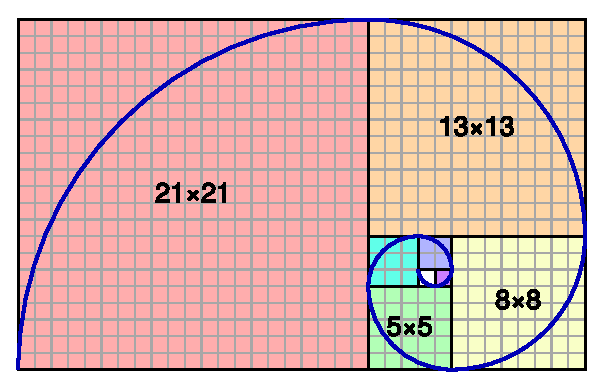
\includegraphics[width=.3\textwidth]{EPS/FibonacciSpiral} \index{spiral of Fibonacci}
%\Caption{ \label{fig:FibonacciSpiral}
A construction called the Fibonacci spiral. Note how it is constructed of squares
that have areas given by the squares of the Fibonacci numbers. In this way, the spiral is smooth and the
radius increases as the Fibonacci numbers (e.g., $8 = 3 + 5$, $13 = 5 + 8$, etc.).
(Adapted from \texttt{\scriptsize https://en.wikipedia.org/wiki/Golden\_spiral})
	
% \end{tcolorbox}
\end{figure}

\BEx %\Exercise
Use the Octave/Matlab command $\texttt{compan(c)}$ to find the companion matrix of the polynomial
coefficients defined by Eq.~\ref{eq:fibonacci}. 
 \index{companion matrix}

\sol{ Using Matlab/Octave:
\texttt{
f=[1, -1, -1]; 
C=compan(f); 
    }
\be
C=
\begin{bmatrix}
1 & 1 \\
1 & 0
\end{bmatrix}
\label{eq:CM-Fibonacci}
\ee
	}%sol
\EEx

\BEx %\Exercise
Find the eigenvalues of matrix $C$.
\index{eigenvalues}

 \sol {
The characteristic equation is
\[
\det
\bbm 1-\lambda & 1 \\ 1 & -\lambda
\ebm
=0
 \]
or
$\lambda^2 -\lambda -1= (\lambda-1/2)^2 -1/4 -1 =0$,
which has roots
 $\lambda_\pm=(1\pm\sqrt{5})/2 \approx \{1.618, -0.618\}$.
}
\EEx

\paragraph{The mean-Fibonacci sequence:}
Suppose that the Fibonacci sequence recursion is replaced by the mean of the last two values--namely, let
\be
f_{n+1} = \frac{f_n + f_{n-1}}{2}.
 \label{eq:avg}
\ee
This seems like a small change. But how does the solution differ?
To answer this question it is helpful to look at the corresponding $2\times 2$ matrix.

\BEx %\Exercise
Find the $2\times 2$ matrix corresponding to Eq.~\ref{eq:avg}.  The $2\times 2$ matrix may be found using the
\emph{companion matrix} method  (see p.~\pageref{sect:CompanionMatrix}).
 \index{companion matrix}

\sol{Using Matlab/Octave code, we have
\\ \\
\texttt{
f=[1, -1/2, -1/2]; \\
C=compan(f); \\
%Rc=eig(C); \\
%Ra=roots(A) \\
    }
\\
which returns
\be
C =
\frac{1}{2}
\begin{bmatrix}
1 & 1 \\
2 & 0
\end{bmatrix}.
\label{eq:avg2x2}
\ee
%{\green \ref{eq:avg2x2}}
	}%sol
\EEx

\BEx %\Exercise
Find the steady-state solution for the mean-Fibonacci, starting from $[1,0]_0$. State the
nature of both solutions.

\sol{By inspection one steady-state solution is $[1,1]^T_\infty$ or $f_n=1$.  To find the full solution, we need to find the two eigenvalues, defined by
\[
\det
\begin{bmatrix}
1/2-\lambda & 1/2 \\
1 & -\lambda
\end{bmatrix}
%\label{eq:avg2x2}
=\lambda^2 -\lambda/2-1/2
= (\lambda-1/4)^2 -(1/4)^2 -1/2 =0.
\]
Thus $\lambda_\pm=
%1/4 \pm 3/4 =
(1\pm3)/4 = [1, -0.5]$. The first solution converges to $1$ while the second solution is $(-1/2)^n$, which changes sign at each time step and
quickly converges to zero. The full solution is given by $\e \Lambda^n \e^{-1} [1,0]^T$
(see Appendix \ref{EigenAnalysis}, p.~\pageref{EigenAnalysis}).
}
\EEx

\index{signal processing, digital}
\paragraph{Relationships to digital signal processing:}
Today we recognize Eq.~\ref{eq:fibonacci} as a discrete difference equation, which is a pre-limit
(pre--Stream 3) recursive form of a differential equation.
The $2\times 2$ matrix form of Eq.~\ref{eq:fibonacci} is an early precursor
to 17th- and 18th-century
developments in linear algebra.  \index{stream 3}
Thus the Greeks' recursive solution for the $\sqrt{2}$ and Bhaskara's solution of
Pell's equation are early precursors to discrete-time signal processing as well as to calculus.

There are strong similarities between Pell's equation and the Pythagorean theorem. 
As we shall see,
%in \S \ref{Chap:NS},
Pell's equation is related to the geometry of a hyperbola, just as the Pythagorean equation is
related to the geometry of a circle.
% \footnote{Sarah: ``You never stated that the PT describes a circle!'' So true. Thanks for pointing this out.
% It also defines a right triangle with the diameter of the circle as the hypotenuse, and three areas given
% by the square of the lengths of the right triangle. The areas of two of these squares must equal the third.}
We shall show, as one might assume, that there is a counterpart to Euclid's formula for the case of Pell's equations,
since these are all conic sections with closely related conic geometry. As we have seen, the solutions
involve $\sqrt{-1}$.  The derivation is a trivial extension of that for Euclid's formula for
Pythagorean triplets.  The early solution of Brahmagupta was not related to this simple formula.
 \index{Brahmagupta}

 %It makes one wonder if Eq.~\ref{eq:PyThm}, written as $x_n^2 + y_n^2 = z_n^2$, with $x_n, y_n, z_n\in\N$,
 %has a $2\times 2$ matrix composition solution. 
 %We shall derive such a relationship in Fig.~\ref{fig:Pell} (p.~\pageref{fig:Pell}). 

%\Exercise Work out the details of this conjecture.  Hint: $z^2=x^2+y^2 = (x+y\jmath)(x-y\jmath)$.
%\sol{ The solution may be found in (???). See Pell's equation for a hint }


%NS3-Pell-Diag.tex, moved out of NS3/Pell.tex to here

\subsection{Diagonalization of a matrix (eigenvalue/eigenvector decomposition)}
As derived in Appendix \ref{EigenAnalysis}, the most efficient way to compute $A^n$ is to
diagonalize the matrix $A$ by finding its eigenvalues and eigenvectors.

%\gray
%\noindent \underline
The eigenvalues $\lambda_k$ and eigenvectors $\vec{e}_k$ of a square matrix $A$ are related by
\be
A\vec{e}_k= \lambda_k \vec{e}_k , \label{eq:ev1}
\ee
such that multiplying an eigenvector $\vec{e}_k$ of $A$ by the matrix $A$ is the same as multiplying by a scalar, $\lambda_k \in \C$ (the corresponding eigenvalue). %An $M\times M$ matrix $A$ may have up to $M$ eigenvalue-eigenvector pairs. 
The complete eigenvalue problem may be written as
 \[
AE=E\Lambda.
 \]
 If $A$ is a $2\times2$ matrix,%BART \footnote{These concepts may be easily extended to higher dimensions.}
  the matrices $E$ and $\Lambda$ (of eigenvectors and eigenvalues, respectively) are%
\[ E =  
\bbm
\vec{e}_1& \vec{e}_2
\ebm
\hspace{.5in}
\text{and}
\hspace{.5in}
\Lambda =
\bbm
\lambda_1 & 0 \\
0 & \lambda_2  
\ebm.
\]
Thus the matrix equation
$AE=
\bbm
A\vec{e}_1 & A\vec{e}_2
\ebm
= \bbm
\lambda_1\vec{e}_1 & \lambda_2\vec{e}_2
\ebm
= E\Lambda$
contains Eq.~\ref{eq:ev1} for each eigenvalue-eigenvector pair.

The diagonalization of the matrix $A$ refers to the fact that the matrix of eigenvalues, $\Lambda$,
has nonzero elements only on the diagonal. The key result is found by  postmultiplication of the
eigenvalue matrix by $E^{-1}$, giving
\begin{equation}
AE E^{-1}= A= E\Lambda E^{-1}.
\end{equation}
If we now take powers of $A$, the $n$th power of $A$ is
\begin{align}
A^n&=(E\Lambda E^{-1})^n  \nonumber\\
&= E\Lambda E^{-1}E\Lambda E^{-1}\cdots E\Lambda E^{-1} \nonumber \\
&= E\Lambda^n E^{-1}.
 \label{eq:diag}
\end{align}
This is a very powerful result because the $n$th power of a diagonal matrix is extremely
easy to calculate:
\[\Lambda^n =
\bbm
\lambda_1^n & 0 \\
0 & \lambda_2^n 
\ebm.
\]
Thus, from Eq.~\ref{eq:diag} we can calculate $A^n$ using only two matrix multiplications:
\[
A^n = E\Lambda^n E^{-1}.
\]

%In matlab this command is \texttt{[E,D]=eig(A)}. %we mention this later

\subsection{Finding the eigenvalues:}
The eigenvalues $\lambda_k$ are determined from Eq.~\ref{eq:ev1}, by factoring out $\vec{e}_k$:
\begin{align*}
A\vec{e}_k &= \lambda_k \vec{e} \\
(A-\lambda_k I)\vec{e}_k &=\vec{0}.
\end{align*}
Matrix $I = [1,0;0,1]^T$ is the identity matrix, having the dimensions of $A$, with elements
$\delta_{ij}$ (i.e., diagonal elements $\delta_{11,22}=1$ and off-diagonal elements $\delta_{12,21}= 0$).

 \index{eigenvalues}
The vector $\vec{e}_k$ is not zero, yet when operated on by $A-\lambda_kI$, the result must be zero.
The only way this can happen is if the operator is degenerate (has no solution)---that is, 
\begin{equation}
\text{det}(A-\lambda I) = \text{det} 
\bbm
(a_{11}-\lambda) & a_{12} \\
a_{21} & (a_{22}-\lambda)
\ebm
= 0 .
\end{equation}
This means that the two equations have the same roots (the equation is degenerate).

This determinant equation results in a second-degree polynomial in $\lambda$:
\[
(a_{11}-\lambda) (a_{22}-\lambda) - a_{12} a_{21} =0,
\]
the roots of which are the eigenvalues of the matrix $A$.

\subsection{Finding the eigenvectors:}
An eigenvector $\vec{e}_k$ can be found for each eigenvalue $\lambda_k$ from Eq.~\ref{eq:ev1},
\[ (A-\lambda_k I)\vec{e}_k =\vec{0}. \]
The left side of the above equation becomes a column vector, where each element is an equation in the
elements of $\vec{e}_k$, set equal to 0 on the right side. These equations are always degenerate,
since the determinant is zero. Thus the two equations have the same slope
 \index{eigenvectors}
\red (Appendix \ref{Apdx:Eigvector}, p.~\pageref{Apdx:Eigvector}).
\black

The vector $\vec{e}_k$ is not zero, yet when operated on by $A-\lambda_kI$, the result must be zero.
The only way this can happen is if the operator is degenerate (has no solution)---that is, 
\begin{equation}
\text{det}(A-\lambda I) = \text{det} 
\bbm
(a_{11}-\lambda) & a_{12} \\
a_{21} & (a_{22}-\lambda)
\ebm
= 0 .
\end{equation}
Solving for the eigenvectors is often confusing because they have arbitrary magnitudes,
$||\vec{e}_k|| = \sqrt{\vec{e}_k \cdot \vec{e}_k} = \sqrt{e_{k,1}^2 + e_{k,2}^2} = d$.
From Eq.~\ref{eq:ev1}, we can determine only the relative magnitudes and signs of the elements of $\vec{e}_k$, so we have to choose a magnitude $d$. It is common practice to normalize each eigenvector to have unit magnitude ($d=1$).

%They determine only the relative magnitudes and signs of the elements of $\vec{e}_k$, meaning the eigenvectors have arbitrary magnitudes,
%$||\vec{e}_k|| = \sqrt{\vec{e}_k \cdot \vec{e}_k} = \sqrt{e_{k,1}^2 + e_{k,2}^2} = d$, which can be confusing. To solve for the eigenvectors, it is necessary to choose a magnitude $d$; typically each eigenvector is \emph{normalized} to have unit magnitude (such that $d=1$).


%NS-3
%\comment
	{%
 \renewcommand{\sol}[1]{} %suppress solution
\index{Assignments: NS-3}

%\setcounter{scratch}{\value{equation}}
\input{NS3/NS3}
%\setcounter{equation}{\value{scratch}}

\newpage
\renewcommand{\sol}[1]{ {\blue{\bf Solution:~}#1}{\gray\tiny$\blacksquare$} }
	}%

%End of chapter 2
\end{document}